\documentclass{sigchi}


% EXAMPLE BEGIN -- HOW TO OVERRIDE THE DEFAULT COPYRIGHT STRIP -- (July 22, 2013 - Paul Baumann)
\toappear{Permission to make digital or hard copies of all or part of this work for personal or classroom use is 	granted without fee provided that copies are not made or distributed for profit or commercial advantage and that copies bear this notice and the full citation on the first page. Copyrights for components of this work owned by others than ACM must be honored. Abstracting with credit is permitted. To copy otherwise, or republish, to post on servers or to redistribute to lists, requires prior specific permission and/or a fee. Request permissions from permissions@acm.org. \\
{\emph{ISWC'15}}, September 7--11, 2015,Osaka, Japan. \\
Copyright \copyright~2014 ACM ISBN/14/04...\$15.00. \\
DOI string from ACM form confirmation}
% EXAMPLE END -- HOW TO OVERRIDE THE DEFAULT COPYRIGHT STRIP -- (July 22, 2013 - Paul Baumann)




% Arabic page numbers for submission. 
% Remove this line to eliminate page numbers for the camera ready copy
% \pagenumbering{arabic}




% Load basic packages
\usepackage{balance}  % to better equalize the last page
\usepackage{graphics} % for EPS, load graphicx instead
\usepackage{times}    % comment if you want LaTeX's default font
\usepackage{url}      % llt: nicely formatted URLs

% llt: Define a global style for URLs, rather that the default one
\makeatletter
\def\url@leostyle{%
  \@ifundefined{selectfont}{\def\UrlFont{\sf}}{\def\UrlFont{\small\bf\ttfamily}}}
\makeatother
\urlstyle{leo}

% To make various LaTeX processors do the right thing with page size.
\def\pprw{8.5in}
\def\pprh{11in}
\special{papersize=\pprw,\pprh}
\setlength{\paperwidth}{\pprw}
\setlength{\paperheight}{\pprh}
\setlength{\pdfpagewidth}{\pprw}
\setlength{\pdfpageheight}{\pprh}

% Make sure hyperref comes last of your loaded packages, 
% to give it a fighting chance of not being over-written, 
% since its job is to redefine many LaTeX commands.
\usepackage[pdftex]{hyperref}
\hypersetup{
pdftitle={SIGCHI Conference Proceedings Format},
pdfauthor={LaTeX},
pdfkeywords={SIGCHI, proceedings, archival format},
bookmarksnumbered,
pdfstartview={FitH},
colorlinks,
citecolor=black,
filecolor=black,
linkcolor=black,
urlcolor=black,
breaklinks=true,
}

% create a shortcut to typeset table headings
\newcommand\tabhead[1]{\small\textbf{#1}}


%%%%%%%%%%%%%%%%%%%%%%%%%%%%%%
%ADDITIONAL PACKAGES
\usepackage{booktabs}
\usepackage[table]{xcolor}% http://ctan.org/pkg/xcolor


% End of preamble. Here it comes the document.
\begin{document}

\title{Skills Assesment for Salsa Dancers \\
Through the Phase Space Representation}

\numberofauthors{3}
\author{
  \alignauthor author 1\\
    \affaddr{Affiliation}\\
    \affaddr{Address}\\
    \email{e-mail address}\\
    \affaddr{Optional phone number}
  \alignauthor author 2\\ %Chris Baber\\
    \affaddr{Affiliation}\\
    \affaddr{Address}\\
    \email{e-mail address}\\
    \affaddr{Optional phone number}    
  \alignauthor author 3\\ %Neil Cooke\\
    \affaddr{Affiliation}\\
    \affaddr{Address}\\
    \email{e-mail address}\\
    \affaddr{Optional phone number}
}

\maketitle

\begin{abstract}
This paper presents a description of the use of time-delay embedding, using Taken's Theorem, 
to analyse data from Inertial Measurement Units mounted on people performing Salsa dance steps.  
The aim of the work is to understand how dexterity can be described in terms of the consistency 
and variability of human activity. To this end, approaches which rely on the definition of 
discrete events or states might not capture dexterity in the same manner. 
The paper shows the application of the approach to expert, intermediate and novice dancers, 
and how these different dancers can be distinguished from the patterns of data the approach produces. 
The paper concludes with a discussion of the potential uses of time-delay embedding for 
Human Activity Recognition using data from wearable sensors.
%%%%%%%%%%%%%%
% RAW IDEAS 
% This paper summarizes work that investigates the formation of the reconstructed state space
% in terms of different values for m and $\tau$
% We are interested in the characterization of the reconstructed state space with the PCA
% in order to propose a metric for skill assessment to Salsa Dancers


\end{abstract}

\keywords{Activity Recognition; b;c;
% 	Guides; instructions; author's kit; conference publications;
% 	keywords should be separated by a semi-colon. \newline
% 	\textcolor{red}{Optional section to be included in your final version, 
%   but strongly encouraged.}
}


\category{I.5.4.}{Pattern Recognition}{Applications}

% \category{H.5.m.}{Information Interfaces and Presentation (e.g. HCI)}{Miscellaneous}
% See: \url{http://www.acm.org/about/class/1998/}
% for more information and the full list of ACM classifiers
% and descriptors. \newline
% \textcolor{red}{Optional section to be included in your final version, 
% but strongly encouraged. On the submission page only the classifiers’ 
% letter-number combination will need to be entered.}



\section{Introduction}

The use of data from wearable sensors to identify human activity is a staple of wearable computer research 
Bulling et al. \cite{Bulling2014}. A core challenge arises from the need to partition these data into segments 
which can be used to label repetitions of discrete events which correlate with specific actions. 
Such an approach draws on signal processing techniques developed to work in the frequency domain and can, 
through stochastic processes, be used to recognise sequences of events.  As Hammerla et al. \cite{Hammerla2011}
note ``[t]herefore information about what subjects are doing is readily available, rendering activity 
segmentation a straight-forward follow up task''. 

Identifying how well the action is performed is more 
challenging. When it comes to studying skilled or dextrous performance, recognition of sequences of events 
might not be sufficient. The reason for this is that dexterity is seldom a matter of performing events 
faster or even of sequencing the events in the same manner as the novice. Rather, the expert segues actions 
into smooth sequences which, through their overlapping and intertwining, become difficult for event-based 
approaches. An alternative is to apply time-series techniques to such data. The focus of this paper is on 
the use of a specific time-series technique to explore a specific aspect of dextrous performance. 
However, the approach can be easily applied to other data and domains. Before explaining the approach, 
the paper begins with a short discussion of dexterity in human performance.

\section{DEXTERITY IN HUMAN PERFORMANCE AND HUMAN ACTIVITY RECOGNITION}
Studies of skilled psychomotor performance indicate the expertise is not simply a matter of performing actions 
in a more consistent manner than novices.  Often the expert is able to produce different but contextually
appropriate actions in a manner that the novice is unable to perform.  This highlights a paradox in human motor 
control: in order to act consistently, people need to produce stable patterns of movement which can be repeated 
efficiently, but these movements also need to exhibit sufficient variability to cope with changes in contextual 
demand. Biomechanics research explains this control of movement in two broad approaches: a common approach is 
to assume that movement is specified in a hierarchy of commands, with a high-level description of a movement 
goal defined in terms of location of end-point for a movement, from which is possible to calculate optimal paths 
for movement; or, less commonly, in terms of parameter optimisation.  For these approaches, consistency is 
explained through the definition of ``motor schema'' which specify the neural commands required to enervate 
the musculoskeletal system to perform a specific action. In such a system, variability in movement arises 
from noise and interference in the translation of motor command to the performance of the movement.  
This means that variability is seen as something which needs to be either ignored or dismissed.  
For Human Activity Recognition, the motor schema view of variability could lead to the assumption that it is 
beneficial to either filter out such ‘noise’ or to define averaged patterns which capture the underlying 
consistency in movement and recognise activity against these patterns. 

An alternative approach sees variability 
in human movement as defined by the originating system. Yamamoto and Gohara \cite{Yamamoto2000} 
define dexterity as ``... the capacity of goal-directed movement to adapt itself to changes in the external 
environment...”  An action involves the coordination of muscles and joints in an efficient manner 
and this raises the ''degrees of freedom``, or ''motor equivalence``, problem \cite{Bernstein1967}.
The motor equivalence problem notes that each joint in the human body has several degrees of freedom in 
the postural angles that it can adopt, and that combining several joint angles in a given movement can result 
in a great many alternative postures, particularly when actions are performed dynamically. While people might 
appear to be making consistent motions in repetitive actions, there is sufficient variability to make it 
difficult to define a single solution to the motor equivalence problem.  The challenge here is to reconstruct 
the originating system in such a way as to allow us to predict the parameters which are being optimised in the 
performance of the movement.  From this perspective, dexterity, or expert performance, could arise from the use 
of specific parameters in the control of movement and the assumption is that experts seek to optimise different 
parameters to novices.  Viewing human motor control in terms of dynamical systems allows researchers to consider 
how expert performance capitalises on the inherent ''noisiness`` of the human movement system.  This approach 
has been particularly fruitful in the field of skill in sports \cite{Davids2003} and we believe that it offers an 
interesting perspective for activity recognition. Applying this assumption to Human Activity Recognition, 
the goal would be to identify the parameters that are being optimised in a data stream that is produced
when activity is performed, rather than in identifying discrete events within that data stream.

In terms of using wearable sensors to study skill,  Ahmadi et al. \cite{Ahmadi2010}, using marker-based 
motion-capture and inertial measurement units (accelerometer and gyroscope) on the person,  showed that skill 
level corresponds to peak values in velocity for shoulder rotation, wrist flexion and upper arm internal 
rotation prior to a tennis serve.  This suggests that the objective classification of skill can be made from 
data acquired from on-body sensors.  Similarly, Baber et al. (submitted) have shown that it is possible to 
distinguish between skill levels for jewellery students performing simple tasks, using sensors embedded in their 
tools.


Previous work on the application of dynamical systems approaches to the study of human activity sought to 
reconcile Bernstein’s \cite{Bernstein1967} concepts with the mathematics of dynamical systems
(Kugler et al., 1980). 
An influential early research paradigm was devleoped by Haken, Kelso and Bunz (Kelso, 1981) \cite{Haken1985} %(Kelso, 1981; Haken et al., 1985).  
In this work, participants performed a very simple task (alternate tapping of index fingers in time to a metronome)
and it was demonstrated that, once the speed exceeds a certain threshold, the two fingers stop moving 
out of phase and move in phase.  This shift is abrupt and indicates a change in attractor state of a 
dynamical system which is seeking to optimise specific order parameters \cite{Beek1995}.
%(Beek et al., 1995).


\begin{figure}[htbp!] 
\centering    
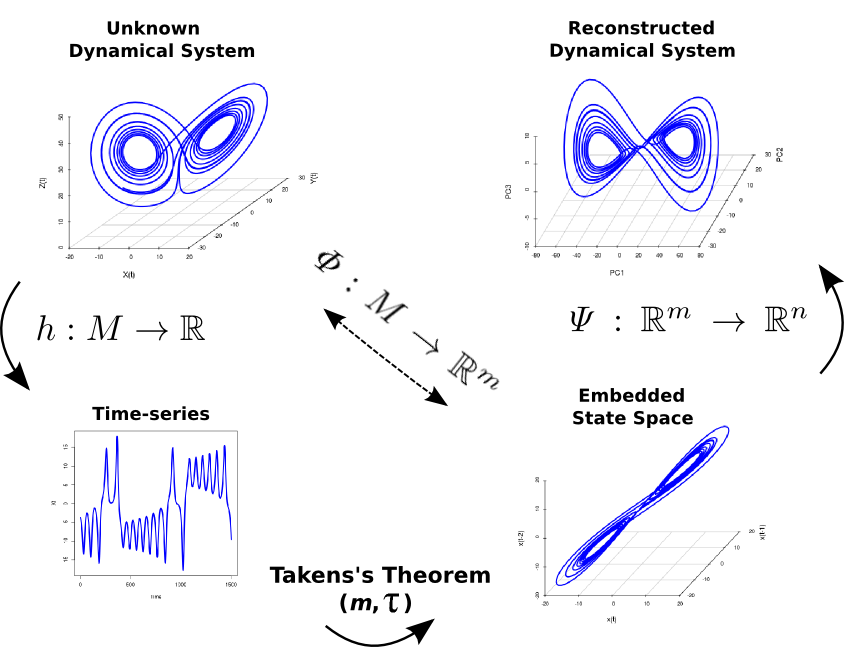
\includegraphics[width=0.45\textwidth]{takens_theorem_v4}
\caption[PA]{The reconstruction problem}
\label{fig:takens_theorem}
\end{figure}



\section{RECOGNISING EXPERTISE IN DANCE}
As Miura et al. \cite{Miura2015} point out ''...how the human motor system produces dance movements in still 
poorly understood.`` A key issue concerns the manner in which experienced dancers solve the degrees of freedom 
problem in the face of changing contextual demands.  Miura et al. \cite{Miura2013} measured muscle activation 
using electromyography (EMG) collected from muscles in the lower limb, for a task requiring participants to 
bounce up and down in time to a metronome beat.  They demonstrated that experienced dancers show much better 
precision in synchronizing movements to beat than non-dancers, i.e., dancers maintained much lower standard 
deviation in temporal deviation against the beat than non-dancers. This result is consistent with work which 
shows that, compared with inexperienced- or non-dancers, trained ballet dancers exhibit superior postural 
stability \cite{Crotts1996} %(Crotts et al., 1996) 
, and show superior ability in position matching of upper limbs \cite{Ramsay2001} %(Ramsey and Riddoch, 2001).  
This suggests that one dimension of dexterity in postural control lies in the manner in which posture is managed 
and controlled.  In addition to dexterity relating to posture, the work on Miura et al. \cite{Miura2013}  %(2013) 
indicates a further dimension, in the manner in which the timing of actions is managed. 

Capturing dance activity through sensors has tended to rely on motion capture \cite{Alexiadis2014} %(Alexiadis and Daras, 2014) 
or sensors mounted on the person \cite{Lynch2005} %(Lynch et al., 2005) 
or in their shoes \cite{Paradiso1997} %(Paradiso and Hu, 1997) 
or from their smartphones  \cite{Wei2014}. %(Wei et al., 2014).  
Much of this work has been concerned with using the dancers’ motion to work with 
multimedia presentations that augment and complement the dance \cite{Griffith1998, Park2006}
%(Grifith and Fernstrom, 1998; Park et al., 2006) 
or as interfacing to a game \cite{Chu2012} %(Chu et al., 2012) 
or commercial games, such as Dance Dance Revolution.  
While the range of sensing technology used in these papers is diverse and the result of the activity 
recognition is varied, it is fair to say that few of the papers have considered variation in how well dance 
is performed.  In their work, Aristidou et al. \cite{Aristidou2014} %(2014) 
have considered the manner in which dance steps conform to a set of defined 
templates that describe steps in terms of three-dimensional rotation (described using quaternions).  
The implication is that a goodness-of-fit can be ascertained to determine how well a dancer performs a step, 
and how any deviation from ‘good’ can be modified through practice. 

For this paper, we are interested in the question of how time-series techniques can provide insight 
into the dexterity of dancers. To this end, we consider the performance of a set of steps from 
Salsa dance and compare untrained, inexperienced and non-dancers in one cohort with experienced dancers on another.





\begin{figure*}[t]
\centering    
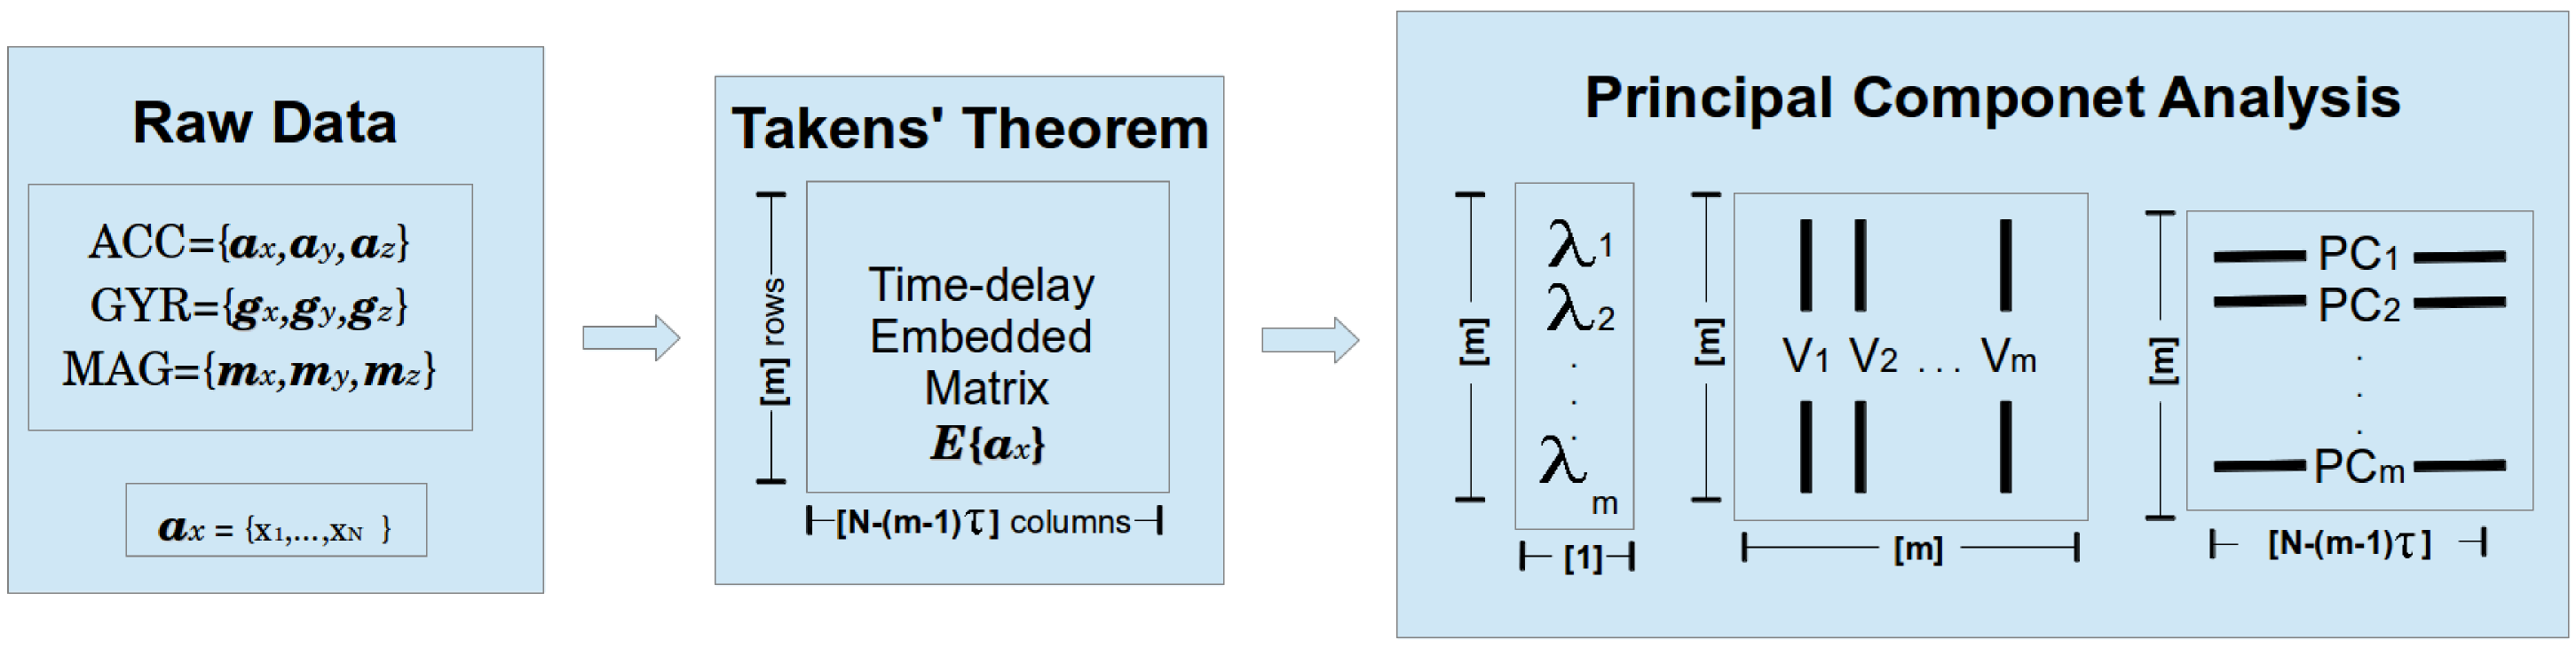
\includegraphics[width=\textwidth]{diagram_v9}
\caption[PA]{Diagram for the Phase Space Reconstruction.}
\label{fig:raw_takens_pca}
\end{figure*}




\section{Phase space representation}
In this work we follow the notation employed in \cite{Uzal2011}.
The purpose of the Takens's Theorem also knowns as time-delay embedding theorem 
is to reconstruct a $D-$dimensional manifold \textbf{M} $s(t)$ of an unknown dynamical 
system from time series $x(t)$ of that system. 
The time series is a sequence $x(t)=h(s(t))$, where $h: M \rightarrow \mathbb{R}^D$
is a measurement function on the unknown dynamical system, being $x(t)$ observable.
The time delay reconstruction in $m$ dimensions with time delay $\tau$ is defined as:
$\overline{x}(t) = (x(t), x(t-\tau),...,x(t-(m-1)\tau))$ which defines a map
$\varPhi: M \rightarrow \mathbb{R}^m$ such that $\overline{x}(t) = \varPhi(s)$.
$\varPsi: \mathbb{R}^m \rightarrow \mathbb{R}^n$ is a further transformation that
is considered as a more general transformation in which for the 
current work we are applying the Principal Component Analyis (PCA) algorithm (Figure \ref{fig:takens_theorem}).
Therefore, our approach is based on the collection 
of raw data from an IMU for triaxial data for accelerometer (ACC), gyroscope (GYR) and magnetometer(MAG) sensors. 
Then, for instance, the time-serie $\textbf{a}_x$ with a lenght of $N$ samples is used to obtain the Time-delay embedded matrix, 
$\boldsymbol{E} a_{x}$, with $m$ rows and $N-(m-1)\tau$ columns. Finally, the PCA algorithm is applied so as to obtain eigenvalues 
($\lambda_1,\ldots,\lambda_m$), eigenvectors ($v_1,\ldots,v_m$) and principal components ($PC_1,\ldots,PC_m$) (Figure \ref{fig:raw_takens_pca}).


\subsection{Determining the minimum embedding dimension}
Although the Takens's Theorem has been used extensevely in gait recognition and walking, running and cycling 
activities some problems are stil remained to be solved.
Sama et al. \cite{Sama2013} estimated the minimal embedded dimension with False Nearest Neighbours (FNN) method.
However, Cao \cite{Cao1997} pointed out that FNN algorithm is subjective to different threshold parameters 
$R_{tol}$ and $A_{tol}$  which lead to different results and FNN method cannot differenciate random series 
from chaotic series. On the other hand, Frank et al. \cite{Frank2010} used a grid search 
to find the embedded parameters, but there are no details about their approach.
Sama et al. \cite{Sama2013} states that the minimal embedding parameters are largely depends on the application at hand, 
nevertheless there is still research to be done to find the minimal embedded parameters ($m$ and $\tau$).

\subsection{$E1(d)$ and $E2(d)$ values}
Cao's method for computing the minimal embedding dimmension is based on the mean values ($E1(d)$, $E2(d)$) of a
modified version of the FNN method, both values are only dependant on $m$ and $\tau$ \cite{Cao1997}.
$E1(d)$ is used to obtain the minimal dimmension and it stops changing when $d$ comes from an attractor.
On the other hand $E2(d)$ is used to distinguish deterministic signals from stochastic signals 
in which case the $E2(d)$ values will be approximately equal to 1 for any $d$.






\section{Experiments}
The data from the  accelerometer, gyro and magnetometer is collected at a 
sampling rate of 50 Hz using four Razor 9DOF Inertial Measurement Units (IMUs) with 
Bluetooth (Adeunis ARF7044).  The IMUs attached to bracelets were worn by participants:
two sensors were located in the front part of the right and left ankle, 
one in the back of the hip and another in back of the neck.

Thirteen male participants with different years of experience in dancing salsa were invited,
one expert dancer (14 years of experience), one intermedium dancer (4 years of experience)
and eleven non-dancers. Participants have been asked to perform two salsa step patterns 
(step 1 = mambo and step 2 = side crossover) repetitively during 20 seconds. 
It is worth noting that non-dancers were asked to mimic a recorded performance of an expert dancer
during a 5 minutes training.


%%%%DIFFERENT TABLEs
% \begin{table}
% \tiny
% 
%   \centering
%   
% \begin{tabular}{l c c c c c c c c c c}
% \toprule
% 
% \multicolumn{11}{c}{Expert} \\
% \cmidrule(r){2-11}
%      & $C_1$  & $C_2$  & $C_3$  & $C_4$  & $C_5$ 
%      & $C_6$  & $C_7$  & $C_8$  & $C_9$  & $C_{10}$ \\
% \midrule
% % Percentega Of Variance
% $\boldsymbol{E} a_{x}$ & 37.83 & 33.82 & 9.42 & 8.98 & 2.93 & 2.19 & 1.49 & 1.24 & 1.05 & 1.01 \\
% $\boldsymbol{E} a_{y}$ & 18.12 & 17.20 & 12.45 & 11.26 & 9.08 & 8.22 & 6.88 & 6.39 & 5.40 & 4.94 \\
% $\boldsymbol{E} a_{z}$ & 29.57 & 25.68 & 17.76 & 11.12 & 5.36 & 3.76 & 2.09 & 1.76 & 1.49 & 1.37 \\
% $\boldsymbol{E} g_{x}$ & 29.98 & 24.89 & 13.73 & 11.73 & 7.50 & 4.27 & 3.23 & 1.97 & 1.39 & 1.26 \\
% $\boldsymbol{E} g_{y}$ & 42.20 & 41.43 & 12.21 & 2.98 & 0.62 & 0.25 & 0.10 & 0.07 & 0.05 & 0.05 \\
% $\boldsymbol{E} g_{z}$ & 40.07 & 36.18 & 13.33 & 6.47 & 1.80 & 0.74 & 0.46 & 0.37 & 0.30 & 0.23 \\
% $\boldsymbol{E} m_{x}$ & 79.18 & 10.81 & 3.98 & 2.43 & 1.21 & 0.83 & 0.61 & 0.43 & 0.29 & 0.19 \\
% $\boldsymbol{E} m_{y}$ & 67.43 & 9.03 & 4.63 & 4.12 & 3.58 & 3.08 & 2.50 & 2.13 & 1.84 & 1.62 \\
% $\boldsymbol{E} m_{z}$ & 66.36 & 28.19 & 3.94 & 0.72 & 0.22 & 0.18 & 0.14 & 0.10 & 0.06 & 0.04 \\
% 
% % mxc1+mxc2=89.99
% % myc1+mzc2=76.46
% % mzc1+mzc2=94.55
% 
% 
% \multicolumn{11}{c}{Intermedium} \\
% \cmidrule(r){2-11}
%      & $C_1$  & $C_2$  & $C_3$  & $C_4$  & $C_5$ 
%      & $C_6$  & $C_7$  & $C_8$  & $C_9$  & $C_{10}$ \\
% \midrule
% % Percentega Of Variance
% $\boldsymbol{E} a_{x}$ & 37.51 & 32.28 & 8.86 & 8.65 & 5.01 & 3.08 & 1.48 & 1.03 & 1.02 & 1.02 \\
% $\boldsymbol{E} a_{y}$ & 20.66 & 20.58 & 14.13 & 13.56 & 8.90 & 5.87 & 4.22 & 4.14 & 3.96 & 3.94 \\
% $\boldsymbol{E} a_{z}$ & 32.77 & 29.85 & 12.47 & 7.60 & 5.03 & 3.35 & 2.70 & 2.21 & 2.02 & 1.95 \\
% $\boldsymbol{E} g_{x}$ & 22.77 & 20.79 & 13.52 & 13.17 & 10.33 & 6.41 & 4.07 & 3.35 & 2.95 & 2.60 \\
% $\boldsymbol{E} g_{y}$ & 46.85 & 40.58 & 9.41 & 1.92 & 0.62 & 0.25 & 0.10 & 0.08 & 0.08 & 0.06 \\
% $\boldsymbol{E} g_{z}$ & 42.43 & 40.21 & 10.60 & 3.45 & 1.61 & 0.73 & 0.37 & 0.22 & 0.18 & 0.14 \\
% $\boldsymbol{E} m_{x}$ & 84.91 & 9.40 & 3.76 & 1.51 & 0.26 & 0.06 & 0.02 & 0.01 & 0.01 & 0.01 \\
% $\boldsymbol{E} m_{y}$ & 64.00 & 28.66 & 5.57 & 1.05 & 0.28 & 0.11 & 0.09 & 0.09 & 0.05 & 0.05 \\
% $\boldsymbol{E} m_{z}$ & 70.24 & 25.43 & 2.99 & 0.49 & 0.17 & 0.14 & 0.13 & 0.12 & 0.12 & 0.12 \\
% 
% 
% 
% % mxc1+mxc2=94.31
% % myc1+mzc2=92.66
% % mzc1+mzc2=95.67
% 
% 
% \multicolumn{11}{c}{Non-dancer} \\
% \cmidrule(r){2-11}
%      & $C_1$  & $C_2$  & $C_3$  & $C_4$  & $C_5$ 
%      & $C_6$  & $C_7$  & $C_8$  & $C_9$  & $C_{10}$ \\
% \midrule
% % Percentega Of Variance
% $\boldsymbol{E} a_{x}$ & 26.41 & 21.57 & 9.45 & 9.24 & 6.61 & 6.52 & 5.69 & 5.40 & 4.82 & 4.22 \\
% $\boldsymbol{E} a_{y}$ & 12.89 & 12.51 & 10.58 & 10.51 & 10.08 & 9.89 & 9.26 & 9.15 & 8.72 & 6.36 \\
% $\boldsymbol{E} a_{z}$ & 15.12 & 14.84 & 12.04 & 10.84 & 9.45 & 9.22 & 8.38 & 6.90 & 6.75 & 6.40 \\
% $\boldsymbol{E} g_{x}$ & 18.45 & 16.66 & 11.21 & 10.63 & 8.41 & 8.33 & 7.96 & 7.00 & 6.10 & 5.20 \\
% $\boldsymbol{E} g_{y}$ & 44.11 & 38.84 & 11.17 & 3.59 & 1.10 & 0.41 & 0.23 & 0.19 & 0.16 & 0.14 \\
% $\boldsymbol{E} g_{z}$ & 37.95 & 37.24 & 10.88 & 3.61 & 2.07 & 1.99 & 1.80 & 1.64 & 1.46 & 1.31 \\
% $\boldsymbol{E} m_{x}$ & 64.24 & 23.82 & 8.91 & 2.29 & 0.40 & 0.11 & 0.06 & 0.04 & 0.036 & 0.03 \\
% $\boldsymbol{E} m_{y}$ & 58.45 & 32.08 & 6.18 & 1.36 & 0.48 & 0.33 & 0.29 & 0.28 & 0.26 & 0.24 \\
% $\boldsymbol{E} m_{z}$ & 66.58 & 27.88 & 4.66 & 0.65 & 0.11 & 0.03 & 0.01 & 0.009 & 0.007 & 0.006 \\
% 
% % mxc1+mxc2=88.06
% % myc1+mzc2=90.53
% % mzc1+mzc2=94.46
% 
% 
% %%%%%%%%%%%%%%%%%%%%%%%%%%%%%%%%%%
% %%%%%%%%%%%%%%%%%%%%%%%%%%%%%%%%%%
% %%%%%%%%%%%%%%%%%%%%%%%%%%%%%%%%%%
% %% NORMALIZED SINGULAR VALUES
% % \multicolumn{11}{c}{Expert} \\
% % \cmidrule(r){2-11}
% %      & $\frac{ \lambda_1 }{ \lambda_1 }$  & $\frac{ \lambda_2 }{ \lambda_1 }$ & $\frac{ \lambda_3 }{ \lambda_1 }$ & $\frac{ \lambda_4 }{ \lambda_1 }$ & $\frac{ \lambda_5 }{ \lambda_1 }$
% %      & $\frac{ \lambda_6 }{ \lambda_1 }$  & $\frac{ \lambda_7 }{ \lambda_1 }$ & $\frac{ \lambda_8 }{ \lambda_1 }$ & $\frac{ \lambda_9 }{ \lambda_1 }$ & $\frac{ \lambda_{10} }{ \lambda_1 }$\\
% % \midrule
% % %normalized singular values: the standard deviations of the principal components 
% % $\boldsymbol{E} a_{x}$ & 1.000 & 0.945 & 0.498 & 0.487 & 0.278 & 0.240 & 0.198 & 0.181 & 0.167 & 0.163 \\
% % $\boldsymbol{E} a_{y}$ & 1.000 & 0.974 & 0.829 & 0.788 & 0.707 & 0.673 & 0.616 & 0.593 & 0.546 & 0.522 \\
% % $\boldsymbol{E} a_{z}$ & 1.000 & 0.931 & 0.774 & 0.613 & 0.425 & 0.356 & 0.265 & 0.244 & 0.224 & 0.215 \\
% % $\boldsymbol{E} g_{x}$ & 1.000 & 0.911 & 0.676 & 0.625 & 0.500 & 0.377 & 0.328 & 0.256 & 0.215 & 0.205 \\
% % $\boldsymbol{E} g_{y}$ & 1.000 & 0.990 & 0.537 & 0.265 & 0.121 & 0.077 & 0.050 & 0.042 & 0.036 & 0.036 \\
% % $\boldsymbol{E} g_{z}$ & 1.000 & 0.950 & 0.576 & 0.401 & 0.212 & 0.136 & 0.107 & 0.097 & 0.087 & 0.077 \\
% % $\boldsymbol{E} m_{x}$ & 1.000 & 0.369 & 0.224 & 0.175 & 0.123 & 0.102 & 0.087 & 0.074 & 0.060 & 0.050 \\
% % $\boldsymbol{E} m_{y}$ & 1.000 & 0.366 & 0.262 & 0.247 & 0.230 & 0.213 & 0.192 & 0.177 & 0.165 & 0.155 \\
% % $\boldsymbol{E} m_{z}$ & 1.000 & 0.651 & 0.243 & 0.104 & 0.057 & 0.052 & 0.046 & 0.039 & 0.032 & 0.027 \\
% 
% % \multicolumn{11}{c}{Intermedium} \\
% % \cmidrule(r){2-11}
% %      & $\frac{ \lambda_1 }{ \lambda_1 }$  & $\frac{ \lambda_2 }{ \lambda_1 }$ & $\frac{ \lambda_3 }{ \lambda_1 }$ & $\frac{ \lambda_4 }{ \lambda_1 }$ & $\frac{ \lambda_5 }{ \lambda_1 }$
% %      & $\frac{ \lambda_6 }{ \lambda_1 }$  & $\frac{ \lambda_7 }{ \lambda_1 }$ & $\frac{ \lambda_8 }{ \lambda_1 }$ & $\frac{ \lambda_9 }{ \lambda_1 }$ & $\frac{ \lambda_{10} }{ \lambda_1 }$\\
% % \midrule
% % $\boldsymbol{E} a_{x}$ & 1.000 & 0.927 & 0.486 & 0.480 & 0.365 & 0.286 & 0.199 & 0.166 & 0.165 & 0.165 \\
% % $\boldsymbol{E} a_{y}$ & 1.000 & 0.997 & 0.827 & 0.810 & 0.656 & 0.533 & 0.452 & 0.447 & 0.437 & 0.436 \\
% % $\boldsymbol{E} a_{z}$ & 1.000 & 0.954 & 0.616 & 0.481 & 0.391 & 0.319 & 0.287 & 0.260 & 0.248 & 0.244 \\
% % $\boldsymbol{E} g_{x}$ & 1.000 & 0.955 & 0.770 & 0.760 & 0.673 & 0.530 & 0.422 & 0.383 & 0.360 & 0.337 \\
% % $\boldsymbol{E} g_{y}$ & 1.000 & 0.930 & 0.448 & 0.202 & 0.115 & 0.073 & 0.047 & 0.043 & 0.042 & 0.038 \\
% % $\boldsymbol{E} g_{z}$ & 1.000 & 0.973 & 0.499 & 0.285 & 0.194 & 0.131 & 0.094 & 0.073 & 0.065 & 0.058 \\
% % $\boldsymbol{E} m_{x}$ & 1.000 & 0.332 & 0.210 & 0.133 & 0.056 & 0.026 & 0.016 & 0.014 & 0.013 & 0.011 \\
% % $\boldsymbol{E} m_{y}$ & 1.000 & 0.669 & 0.295 & 0.128 & 0.066 & 0.043 & 0.039 & 0.037 & 0.029 & 0.028 \\
% % $\boldsymbol{E} m_{z}$ & 1.000 & 0.601 & 0.206 & 0.083 & 0.049 & 0.044 & 0.043 & 0.042 & 0.042 & 0.042 \\
% 
% % 
% % \multicolumn{11}{c}{Non-dancer} \\
% % \cmidrule(r){2-11}
% %      & $\frac{ \lambda_1 }{ \lambda_1 }$  & $\frac{ \lambda_2 }{ \lambda_1 }$ & $\frac{ \lambda_3 }{ \lambda_1 }$ & $\frac{ \lambda_4 }{ \lambda_1 }$ & $\frac{ \lambda_5 }{ \lambda_1 }$
% %      & $\frac{ \lambda_6 }{ \lambda_1 }$  & $\frac{ \lambda_7 }{ \lambda_1 }$ & $\frac{ \lambda_8 }{ \lambda_1 }$ & $\frac{ \lambda_9 }{ \lambda_1 }$ & $\frac{ \lambda_{10} }{ \lambda_1 }$\\
% % \midrule
% % $\boldsymbol{E} a_{x}$ & 1.000 & 0.903 & 0.598 & 0.591 & 0.500 & 0.497 & 0.464 & 0.452 & 0.427 & 0.400 \\
% % $\boldsymbol{E} a_{y}$ & 1.000 & 0.985 & 0.905 & 0.902 & 0.884 & 0.875 & 0.847 & 0.842 & 0.822 & 0.702 \\
% % $\boldsymbol{E} a_{z}$ & 1.000 & 0.990 & 0.892 & 0.846 & 0.790 & 0.781 & 0.744 & 0.675 & 0.668 & 0.650 \\
% % $\boldsymbol{E} g_{x}$ & 1.000 & 0.950 & 0.779 & 0.759 & 0.675 & 0.672 & 0.657 & 0.616 & 0.575 & 0.530 \\
% % $\boldsymbol{E} g_{y}$ & 1.000 & 0.938 & 0.503 & 0.285 & 0.158 & 0.097 & 0.072 & 0.067 & 0.061 & 0.058 \\
% % $\boldsymbol{E} g_{z}$ & 1.000 & 0.990 & 0.535 & 0.308 & 0.233 & 0.229 & 0.218 & 0.208 & 0.196 & 0.185 \\
% % $\boldsymbol{E} m_{x}$ & 1.000 & 0.608 & 0.372 & 0.189 & 0.079 & 0.042 & 0.031 & 0.027 & 0.023 & 0.023 \\
% % $\boldsymbol{E} m_{y}$ & 1.000 & 0.740 & 0.325 & 0.153 & 0.091 & 0.075 & 0.070 & 0.070 & 0.067 & 0.064 \\
% % $\boldsymbol{E} m_{z}$ & 1.000 & 0.647 & 0.264 & 0.099 & 0.041 & 0.024 & 0.015 & 0.011 & 0.010 & 0.009 \\
% %% NORMALIZED SINGULAR VALUES
% %%%%%%%%%%%%%%%%%%%%%%%%%%%%%%%%%%
% %%%%%%%%%%%%%%%%%%%%%%%%%%%%%%%%%%
% %%%%%%%%%%%%%%%%%%%%%%%%%%%%%%%%%%
% 
% \bottomrule
% \end{tabular}
% 
% %   \caption{Normalized eigenvalues values for the expert, intermediate and non-dancer users.
% %   Data from each axis of the IMU $\#0$ on the step 1 is used to compute this eigenvalues.}
%   \caption{PCA's Percentages of variances from each embedded matrix axis of the IMU
%    for expert, intermediate and non-dancer users performing the step 1.}
%   \label{tab:table1}
% \end{table}





%http://tex.stackexchange.com/questions/110739/table-formatting
\begin{table}
\tiny

  \centering
  
\begin{tabular}{l c c c c c c }
\toprule



& \multicolumn{6}{c}{Expert} \\
\cmidrule(r){2-7}

& \multicolumn{3}{c}{Step 1} & \multicolumn{3}{c}{Step 2}\\
\cmidrule(lr){2-4} \cmidrule(lr){5-7}

     & $C_1$  & $C_2$  & $C_1+C_2$  & $C_1$  & $C_2$  & $C_1+C_2$  \\
\midrule
% Percentega Of Variance

$\boldsymbol{E} a_{x}$ & 37.83 & 33.82 & 67.65 & 37.83 & 31.27 & 69.11 \\
$\boldsymbol{E} a_{y}$ & 18.12 & 17.20 & 35.32 & 30.49 & 23.99 & 54.48 \\
$\boldsymbol{E} a_{z}$ & 29.57 & 25.68 & 55.25 & 21.24 & 21.09 & 42.34 \\
$\boldsymbol{E} g_{x}$ & 29.98 & 24.89 & 54.87 & 32.73 & 27.68 & 60.42 \\
$\boldsymbol{E} g_{y}$ & 42.20 & 41.43 & 83.63 & 40.61 & 36.43 & 77.04 \\
$\boldsymbol{E} g_{z}$ & 40.07 & 36.18 & 76.25 & 43.32 & 41.38 & 84.71 \\
$\boldsymbol{E} m_{x}$ & 79.18 & 10.81 & 89.99 & 82.13 & 10.42 & 92.56 \\
$\boldsymbol{E} m_{y}$ & 67.43 & 9.03 & 76.46 & 73.31 & 21.00 & \cellcolor{blue!25}94.31 \\
$\boldsymbol{E} m_{z}$ & 66.36 & 28.19 & \cellcolor{blue!25}94.55 & 61.58 & 25.78 & 87.37   \\



\\
\\
& \multicolumn{6}{c}{Intermedium} \\
\cmidrule(r){2-7}

& \multicolumn{3}{c}{Step 1} & \multicolumn{3}{c}{Step 2}\\
\cmidrule(lr){2-4} \cmidrule(lr){5-7}
     & $C_1$  & $C_2$  & $C_1+C_2$  & $C_1$  & $C_2$  & $C_1+C_2$  \\
\midrule

$\boldsymbol{E} a_{x}$ & 37.51 & 32.28 & 69.79 & 23.11 & 22.17 & 45.28 \\
$\boldsymbol{E} a_{y}$ & 20.66 & 20.58 & 41.24 & 23.07 & 18.15 & 41.23 \\
$\boldsymbol{E} a_{z}$ & 32.77 & 29.85 & 62.62 & 14.35 & 13.65 & 28.00 \\
$\boldsymbol{E} g_{x}$ & 22.77 & 20.79 & 43.56 & 18.58 & 17.49 & 36.08 \\
$\boldsymbol{E} g_{y}$ & 46.85 & 40.58 & 87.43 & 40.32 & 39.21 & 79.53 \\
$\boldsymbol{E} g_{z}$ & 42.43 & 40.21 & 82.64 & 53.13 & 32.90 & 86.04 \\
$\boldsymbol{E} m_{x}$ & 84.91 & 9.40 & 94.31 & 81.80 & 15.01 & \cellcolor{blue!25}96.81 \\
$\boldsymbol{E} m_{y}$ & 64.00 & 28.66 & 92.66 & 77.41 & 18.17 & 95.59 \\
$\boldsymbol{E} m_{z}$ & 70.24 & 25.43 & \cellcolor{blue!25}95.67 & 79.29 & 16.45 & 95.75  \\


\\
\\
& \multicolumn{6}{c}{Non-dancer} \\
\cmidrule(r){2-7}

& \multicolumn{3}{c}{Step 1} & \multicolumn{3}{c}{Step 2}\\
\cmidrule(lr){2-4} \cmidrule(lr){5-7}
     & $C_1$  & $C_2$  & $C_1+C_2$  & $C_1$  & $C_2$  & $C_1+C_2$  \\
\midrule

$\boldsymbol{E} a_{x}$ & 26.41 & 21.57 & 47.98 & 31.27 & 23.92 & 55.20  \\
$\boldsymbol{E} a_{y}$ & 12.89 & 12.51 & 25.4 & 19.79 & 18.88 & 38.68 \\
$\boldsymbol{E} a_{z}$ & 15.12 & 14.84 & 29.96 & 20.22 & 18.75 & 38.98 \\
$\boldsymbol{E} g_{x}$ & 18.45 & 16.66 & 35.11 & 18.78 & 15.12 & 33.90 \\
$\boldsymbol{E} g_{y}$ & 44.11 & 38.84 & 82.95 & 43.20 & 33.99 & 77.20 \\
$\boldsymbol{E} g_{z}$ & 37.95 & 37.24 & 75.19 & 49.76 & 30.21 & 79.97 \\
$\boldsymbol{E} m_{x}$ & 64.24 & 23.82 & 88.06 & 83.79 & 12.43 & 96.23 \\
$\boldsymbol{E} m_{y}$ & 58.45 & 32.08 & 90.53 & 85.71 & 12.06 & \cellcolor{blue!25}97.77 \\
$\boldsymbol{E} m_{z}$ & 66.58 & 27.88 & \cellcolor{blue!25}94.46 & 72.99 & 20.96 & 93.96 \\

\bottomrule
\end{tabular}

%   \caption{Normalized eigenvalues values for the expert, intermediate and non-dancer users.
%   Data from each axis of the IMU $\#0$ on the step 1 is used to compute this eigenvalues.}
  \caption{PCA's percentages of variances of first two components and its addition.
  %Data is taken from each embedded matrix axis of the IMU for expert, intermediate and non-dancer users performing the step 1 and step 2.
  Colored cells represent the maxium percentange of variation of the fist two components.}
  \label{tab:table1}
\end{table}




\section{Results}



Data from the inertial sensor for left ankle of the expert dancer were used
to compute the $E1(d)$ and $E2(d)$ values. From $E1(d)$ values 
(Figures~\ref{fig:e1acc},~\ref{fig:e1gyr} and ~\ref{fig:e1mag})
one can notice that the minimal value for the embedded dimmension is approximately
equal to $m=10$. It is important to note that neither the axis of the intertial sensor 
nor the time-delay values are a factor for having different embedded dimension parameters.
On the other hand, from $E2(d)$ values (Figures~\ref{fig:e2acc},~\ref{fig:e2gyr} and ~\ref{fig:e2mag})
one can appreciate that the accelerometer data is more random since their values are closer to 1
which is also the case for the x-axis in the gyroscope and magnetometer sensor. 
Fortunately, y and z axis in the gyroscope and magnetometer provide more deterministic data.

Considering the fact that different $\tau$ values provide approximately the same minimal embeding dimension ($m=10$),
we choose $\tau = 1$. Then, as depicted in Figure \ref{fig:raw_takens_pca}, the Takens' Theorem is computed 
with $m=10$ and $\tau = 1$ for each of the axis of the IMU. 
Table~\ref{tab:table1} illustrates the first two components of all axis for step 1 and step 2 from
expert, intermedium and non-dancer participants.
Table~\ref{tab:table1} help us to choose the first two components of the magnetometer data in the z-axis,
since these has the highest variance for step 1. In the case of the step 2, we select y-axis of the magnetometer 
given that expert and the novice have the highest variance in this variable.


Figure ~\ref{fig:skills} illustrates the 2-D reconstructed state space
for the non-dancer, intermediate and experte dancers which visually help us to
distinguish different levels of skills.

We also illustrate the problem of the minimal embedded parameters by 
presenting different reconstructed state spaces in Figure ~\ref{fig:takens}.


  \begin{figure}[htbp!] 
  \centering    
  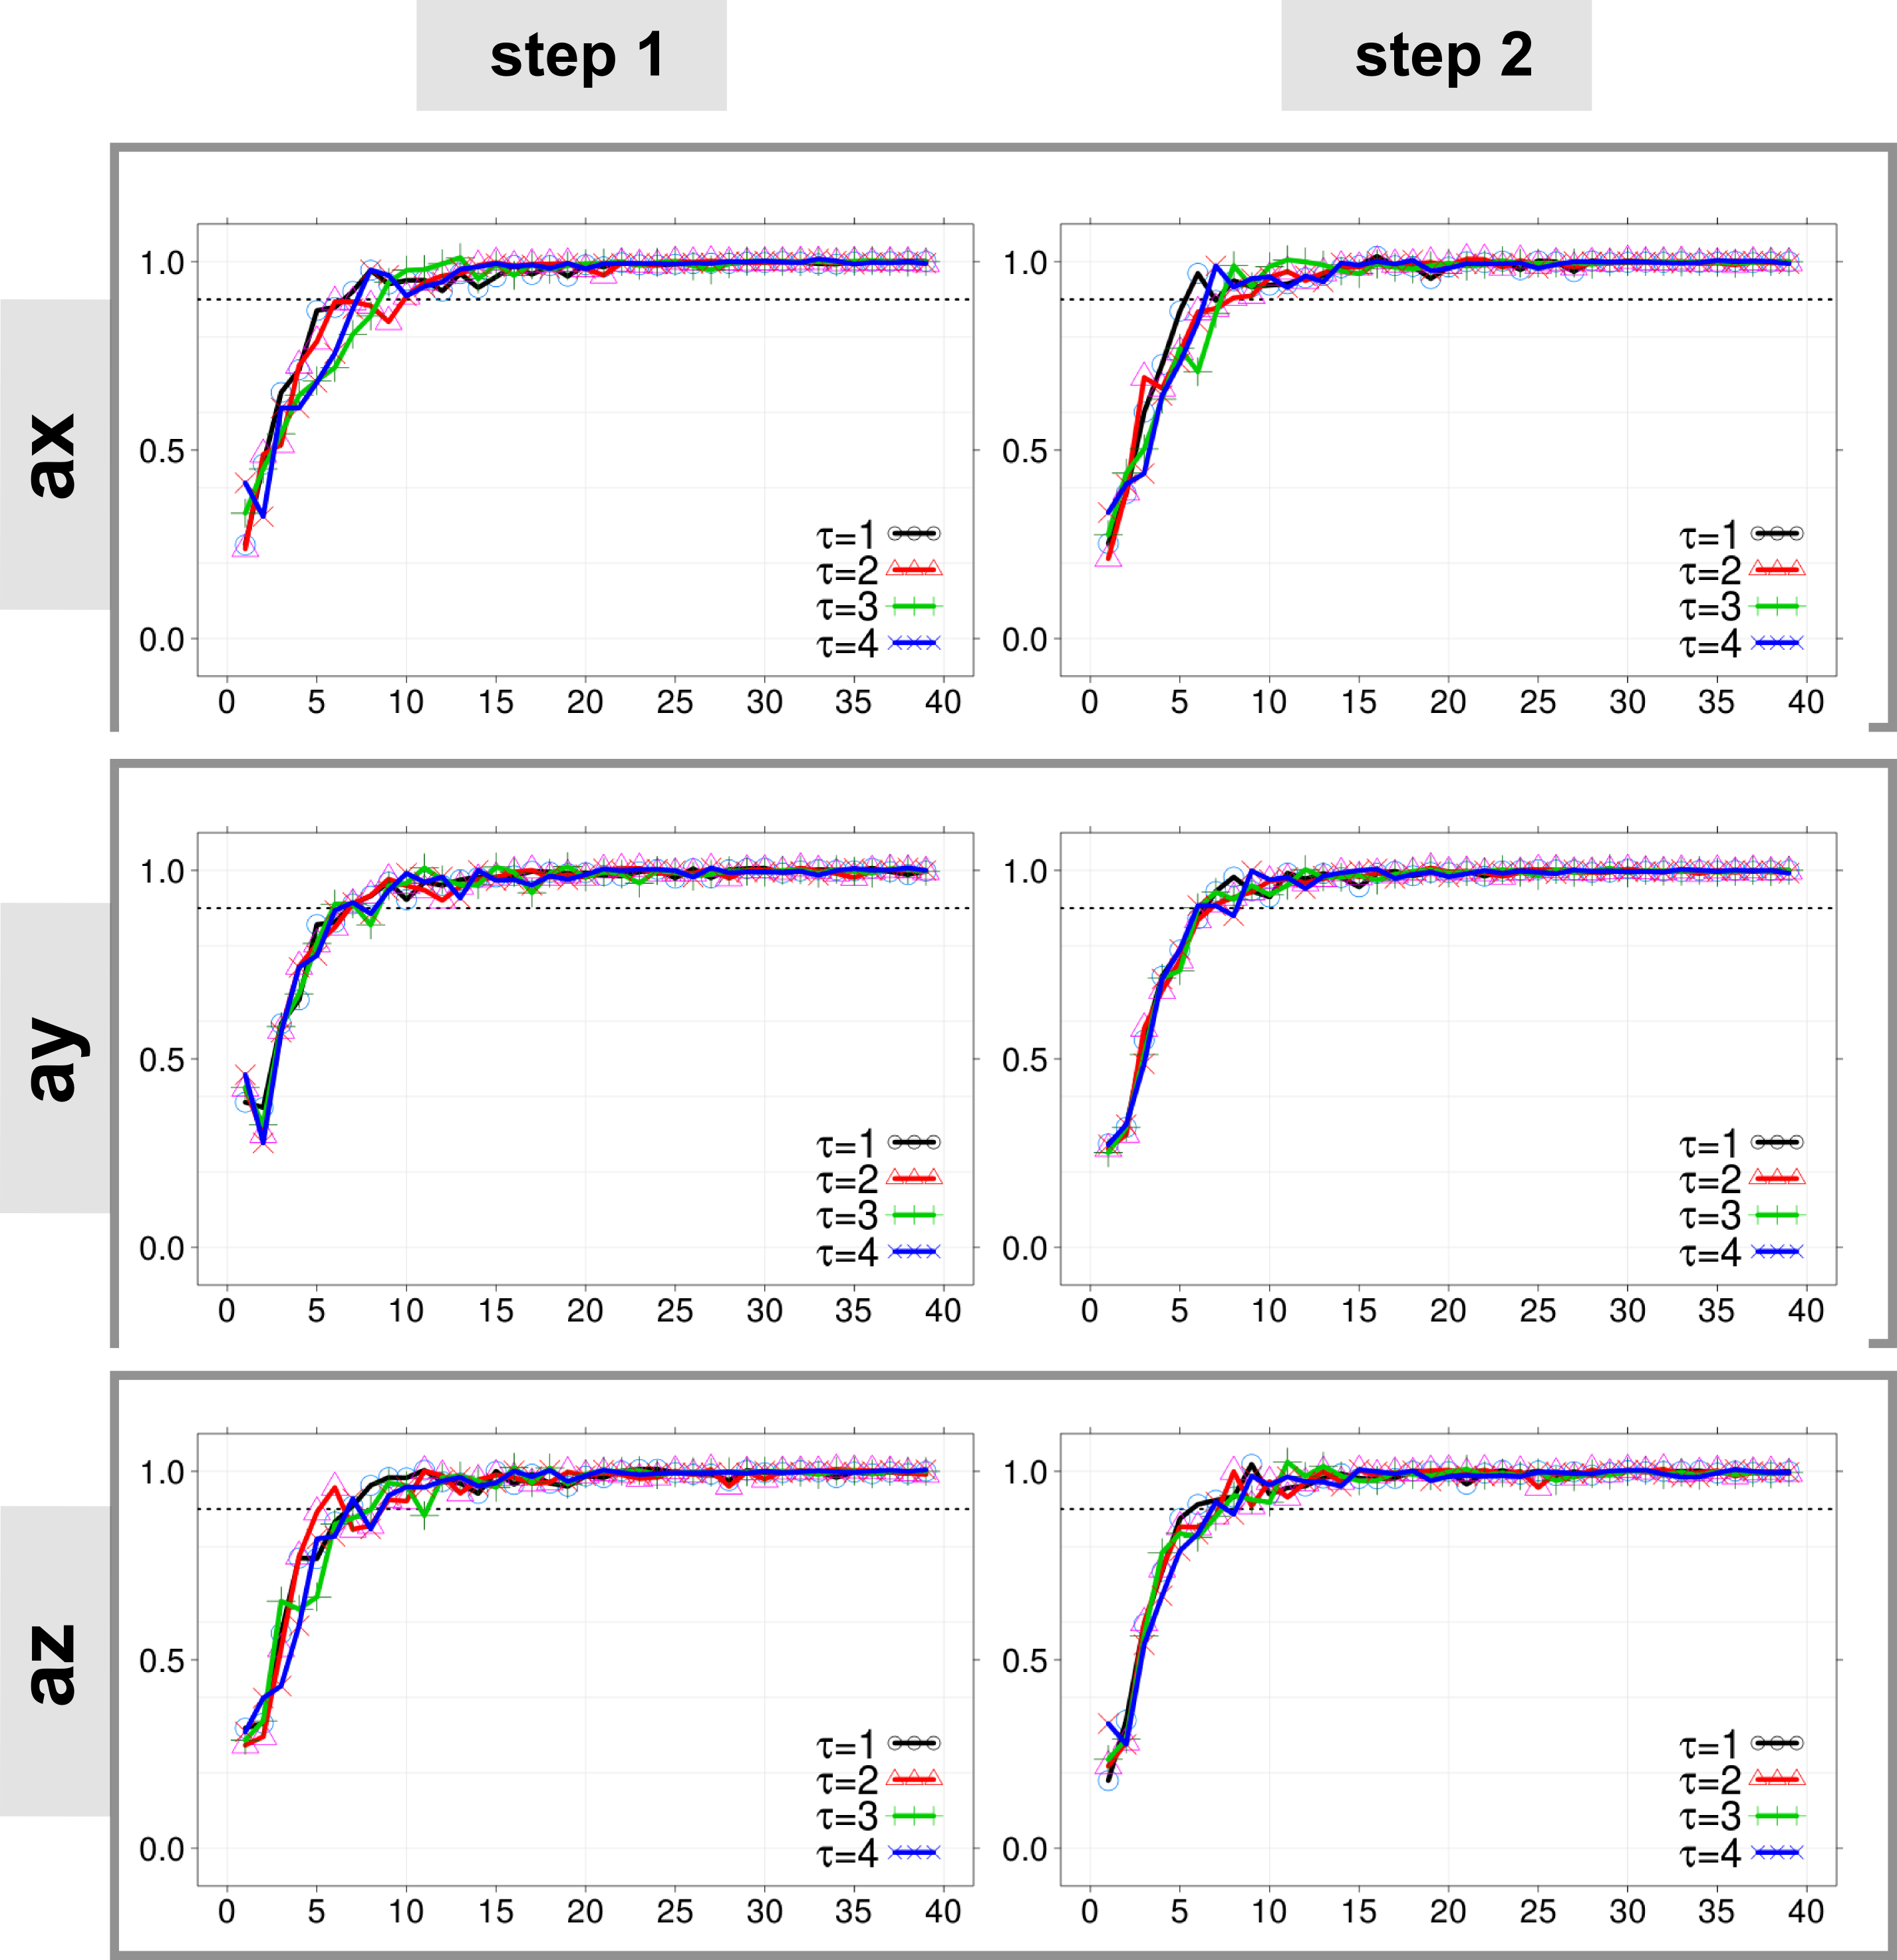
\includegraphics[width=0.45\textwidth]{e1_acc_expert}
  \caption[PA]{$E1(d)$ values for $\tau=1,2,3,4$ with $0 \leq d \leq 40$
  from the triaxial accelerometer of the expert dancer for two steps.}
  \label{fig:e1acc}
  \end{figure}
  

    \begin{figure}[htbp!] 
  \centering    
  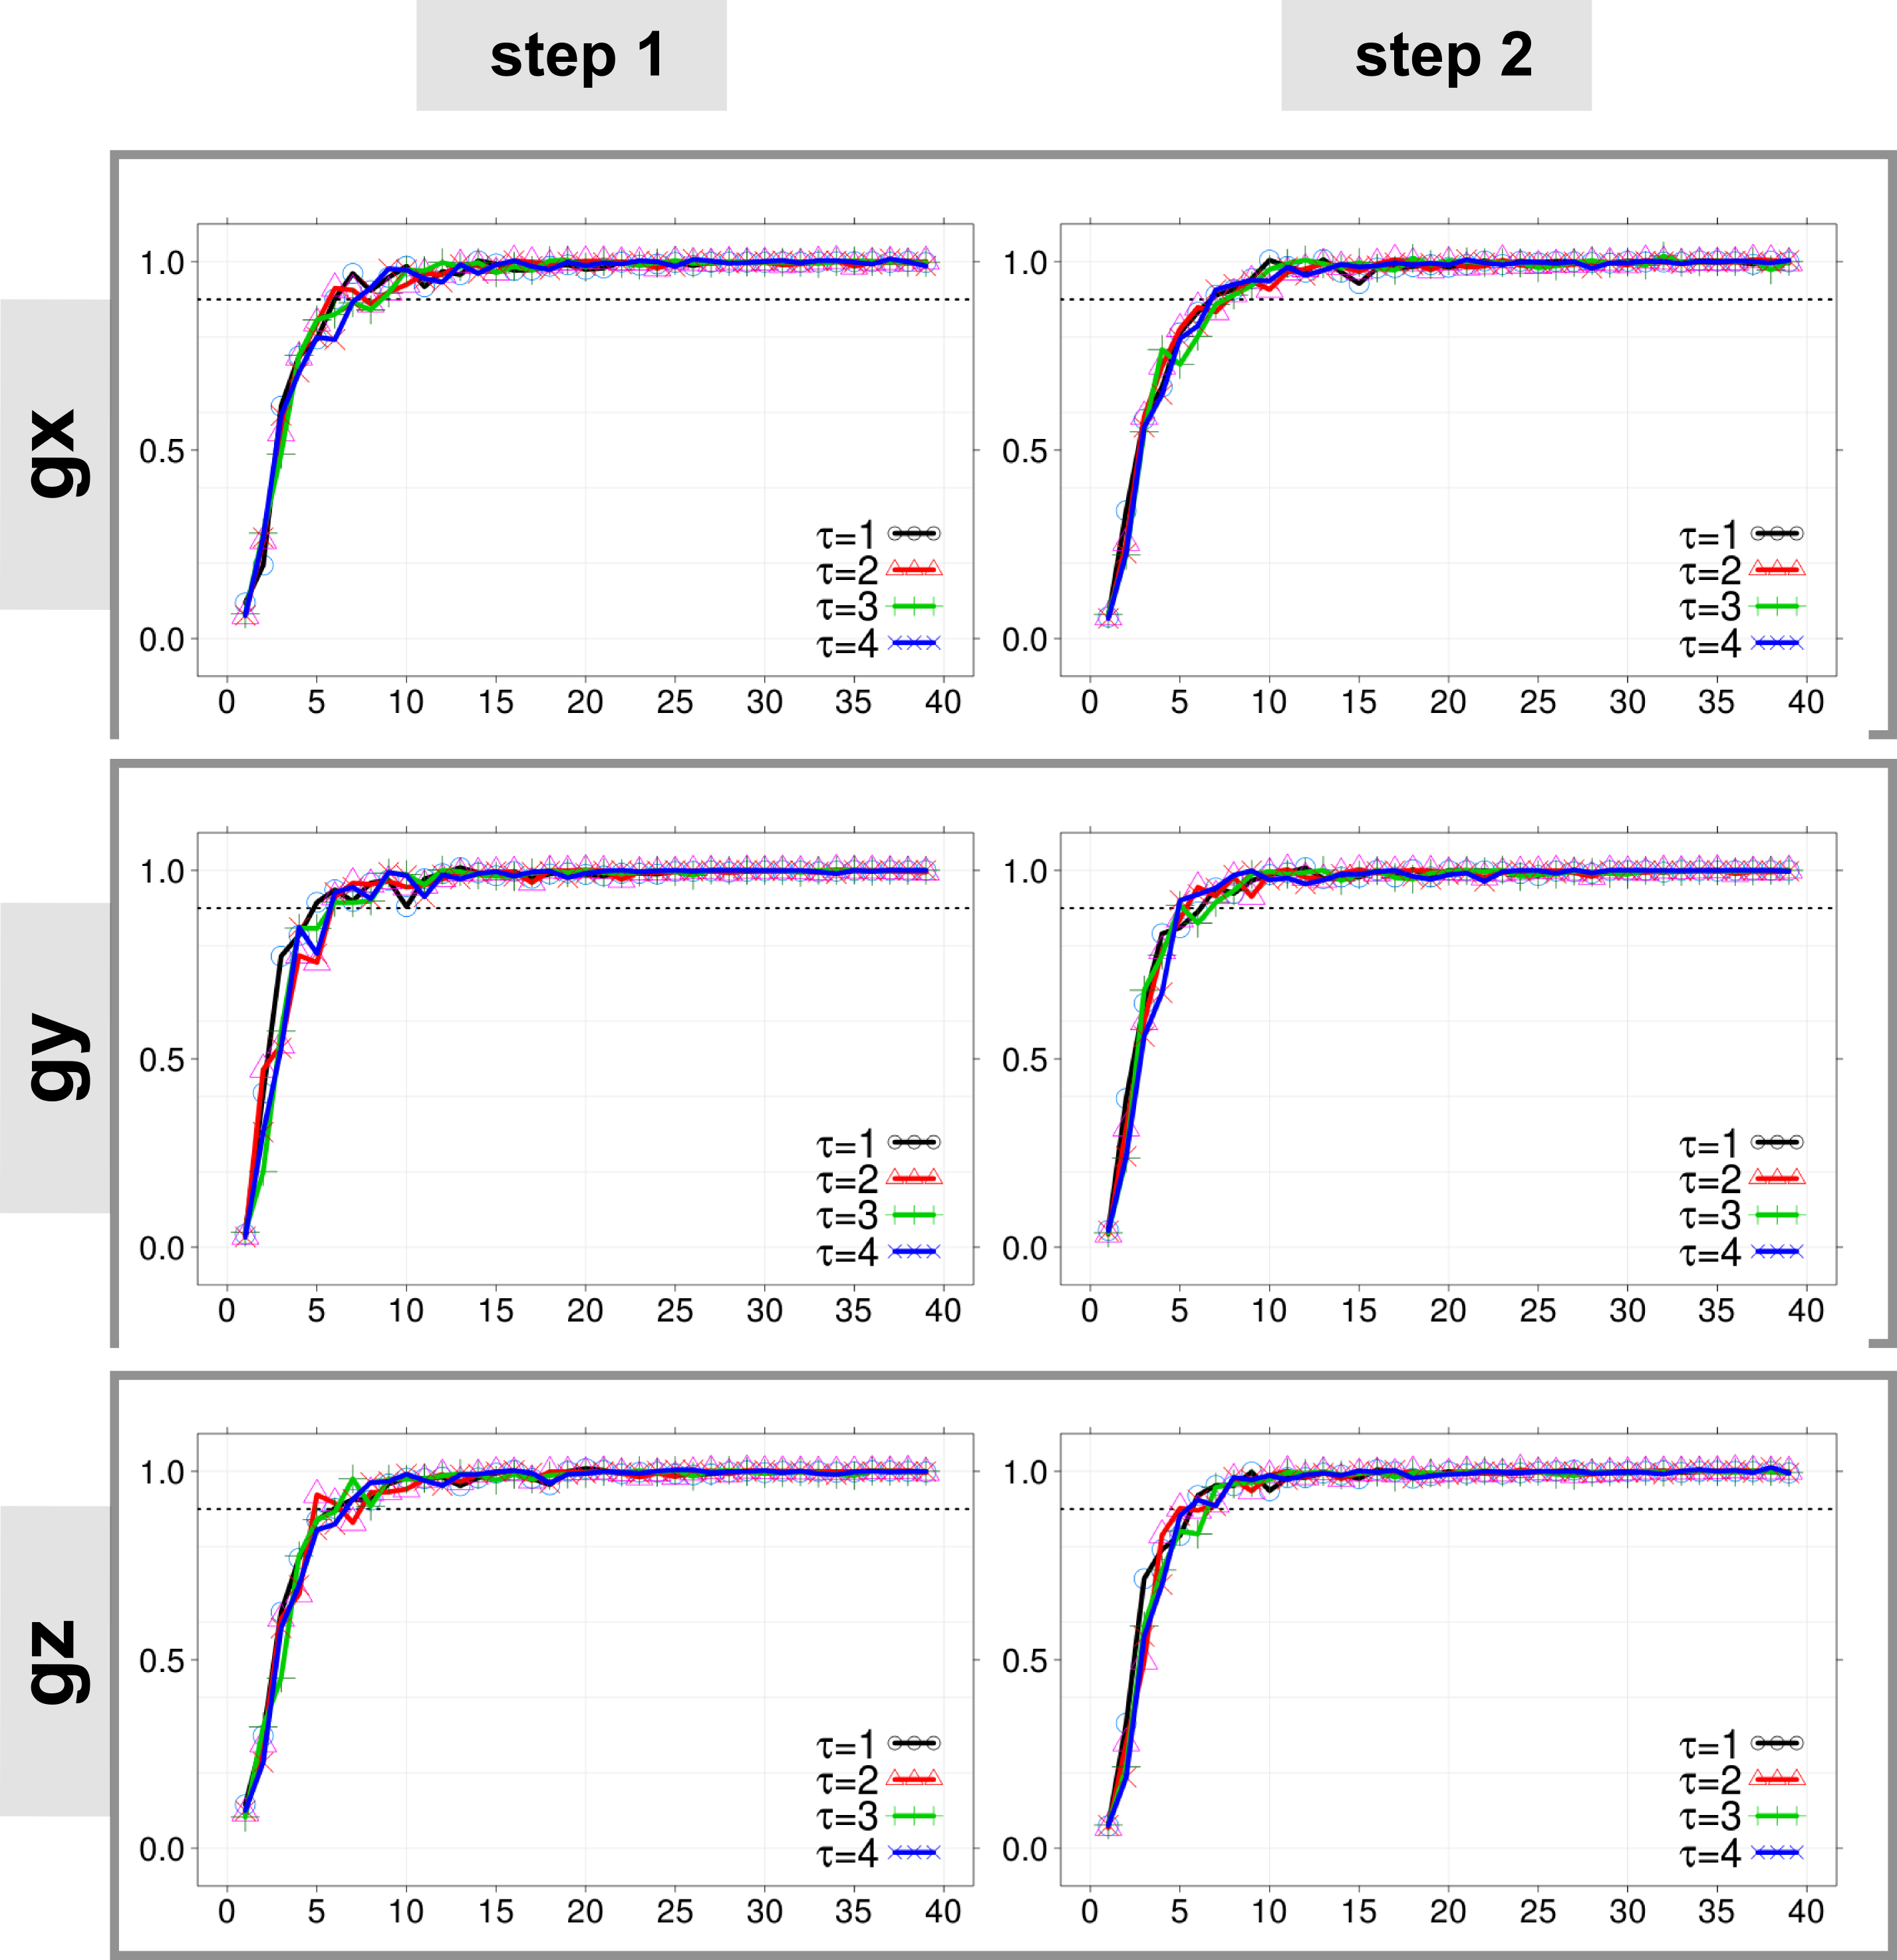
\includegraphics[width=0.45\textwidth]{e1_gyr_expert}
  \caption[PA]{$E1(d)$ values for $\tau=1,2,3,4$ with $0 \leq d \leq 40$
  from the triaxial gyroscope of the expert dancer for two steps.}
  \label{fig:e1gyr}
  \end{figure}
  
    \begin{figure}[htbp!] 
  \centering    
  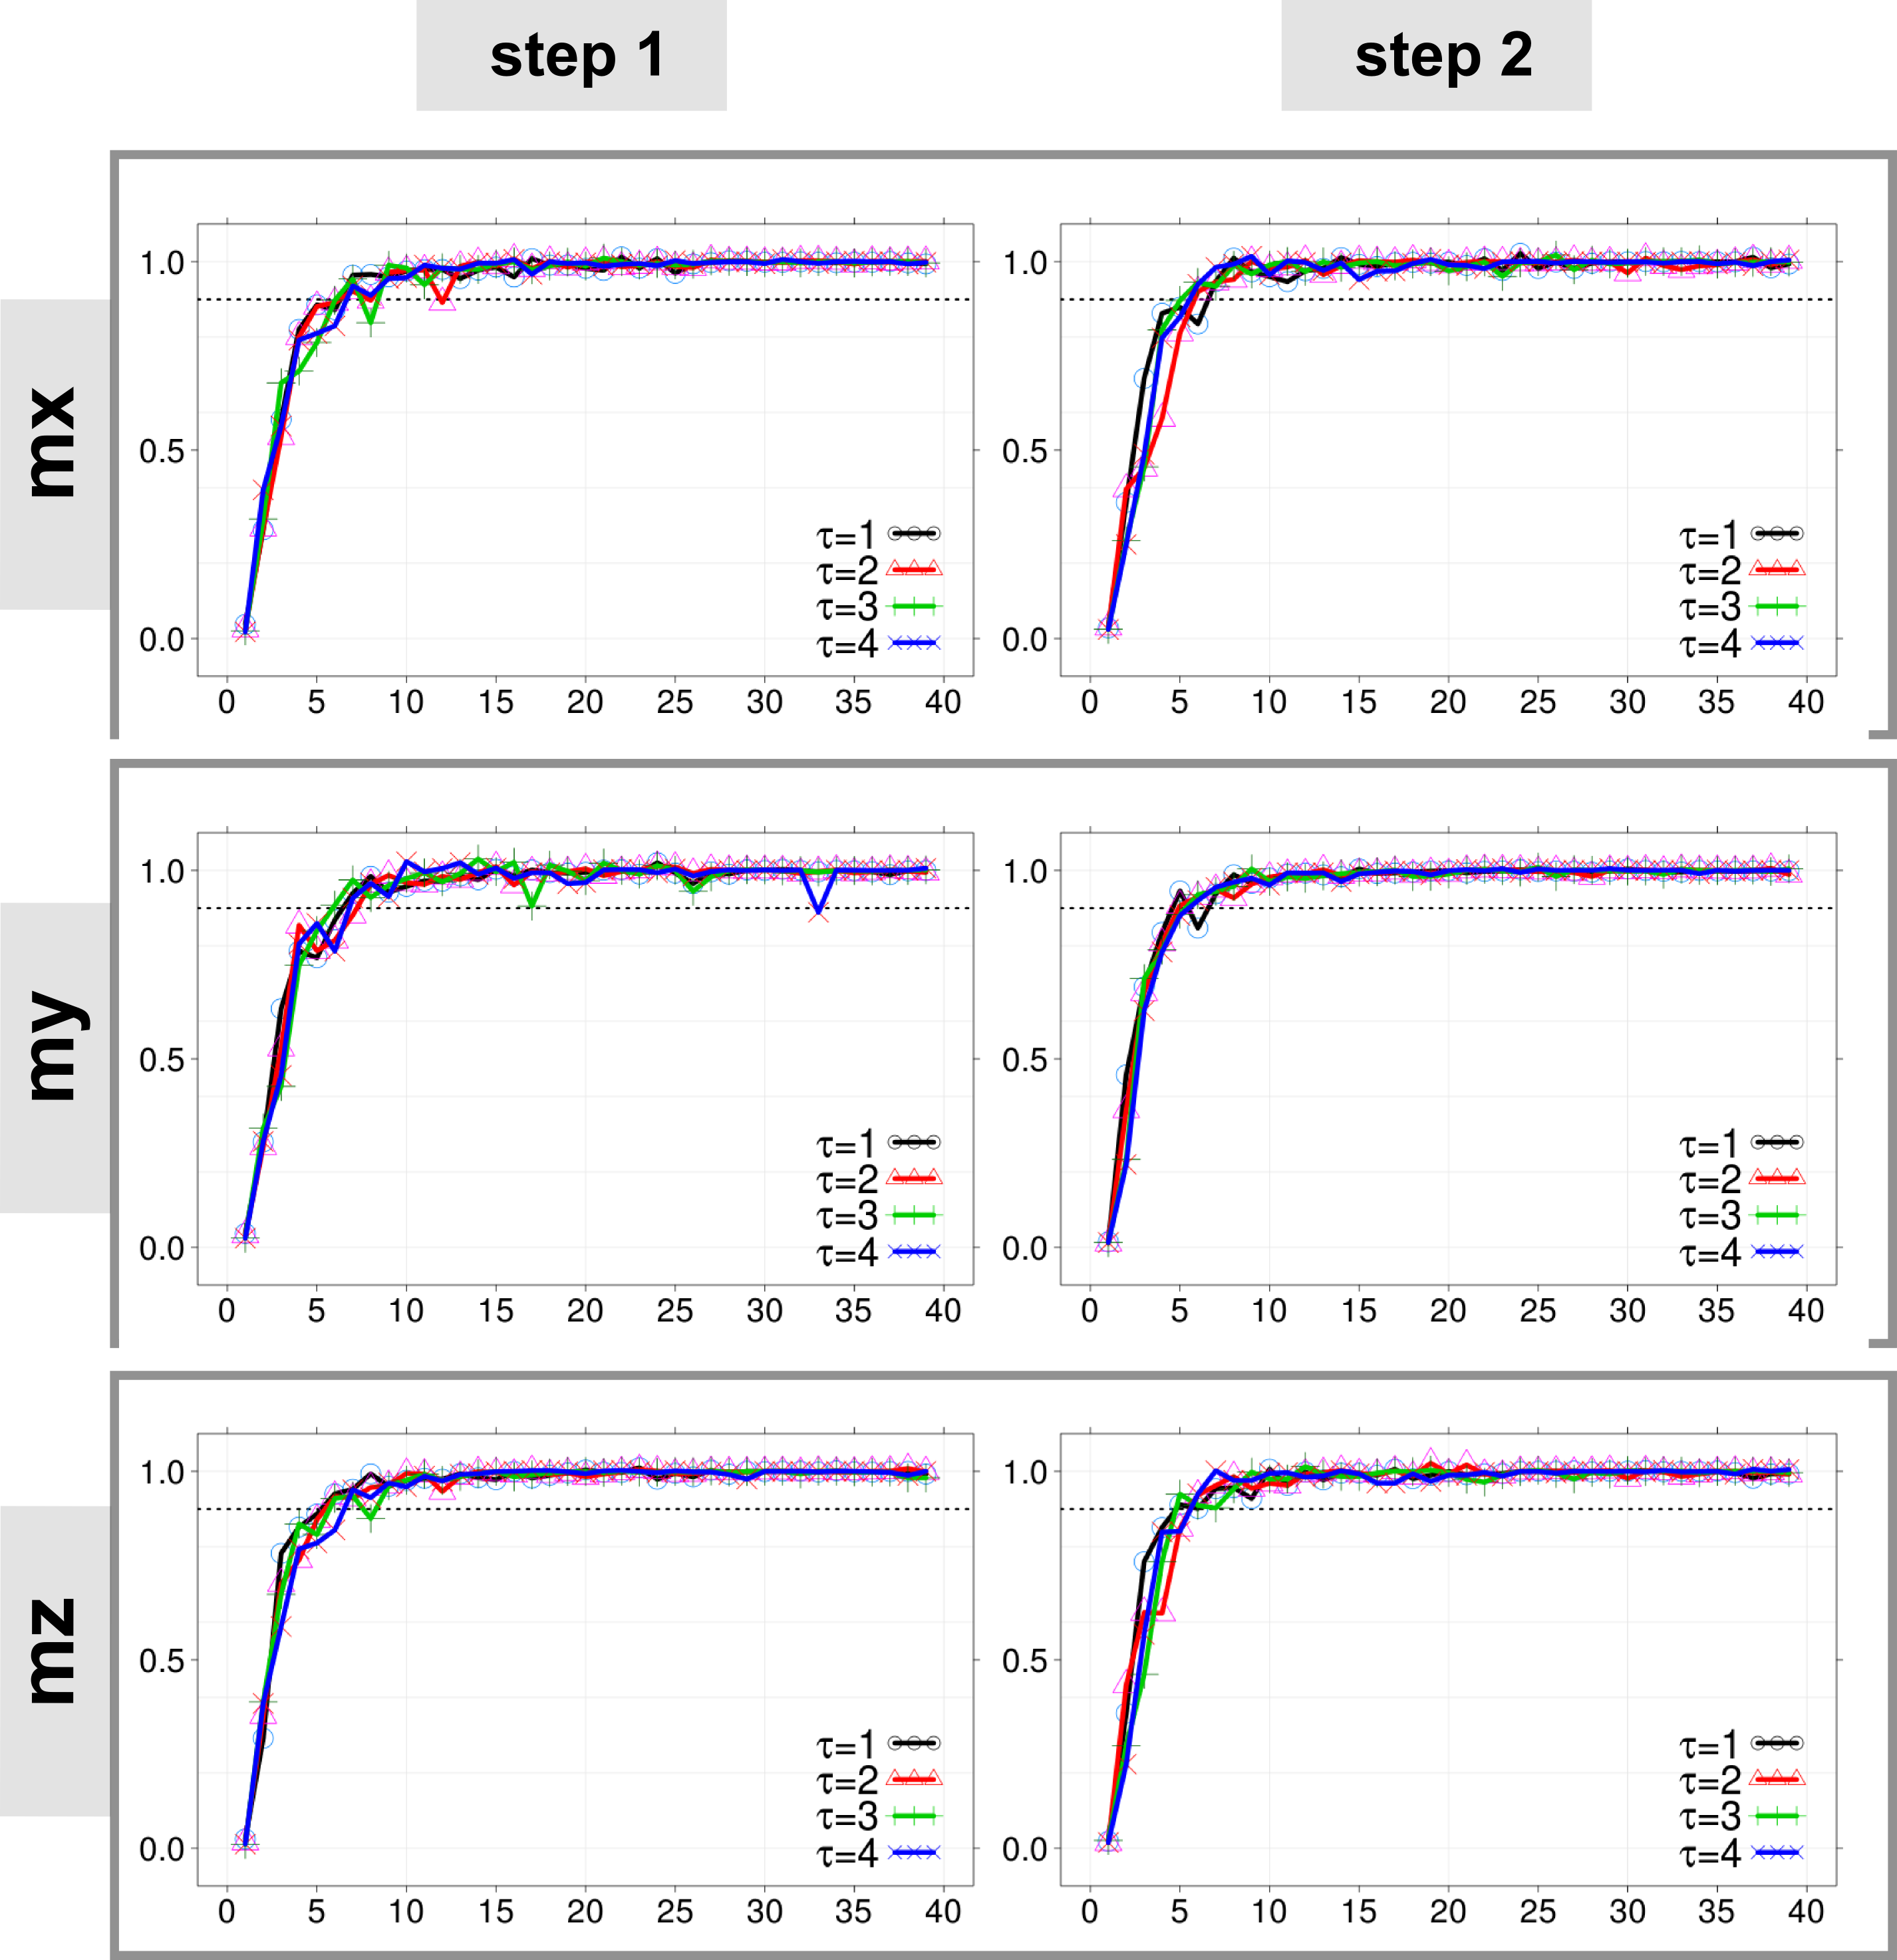
\includegraphics[width=0.45\textwidth]{e1_mag_expert}
  \caption[PA]{$E1(d)$ values for $\tau=1,2,3,4$ with $0 \leq d \leq 40$
  from the triaxial magnetometer of the expert dancer for two steps.}
  \label{fig:e1mag}
  \end{figure}
  
  \begin{figure}[htbp!] 
  \centering    
  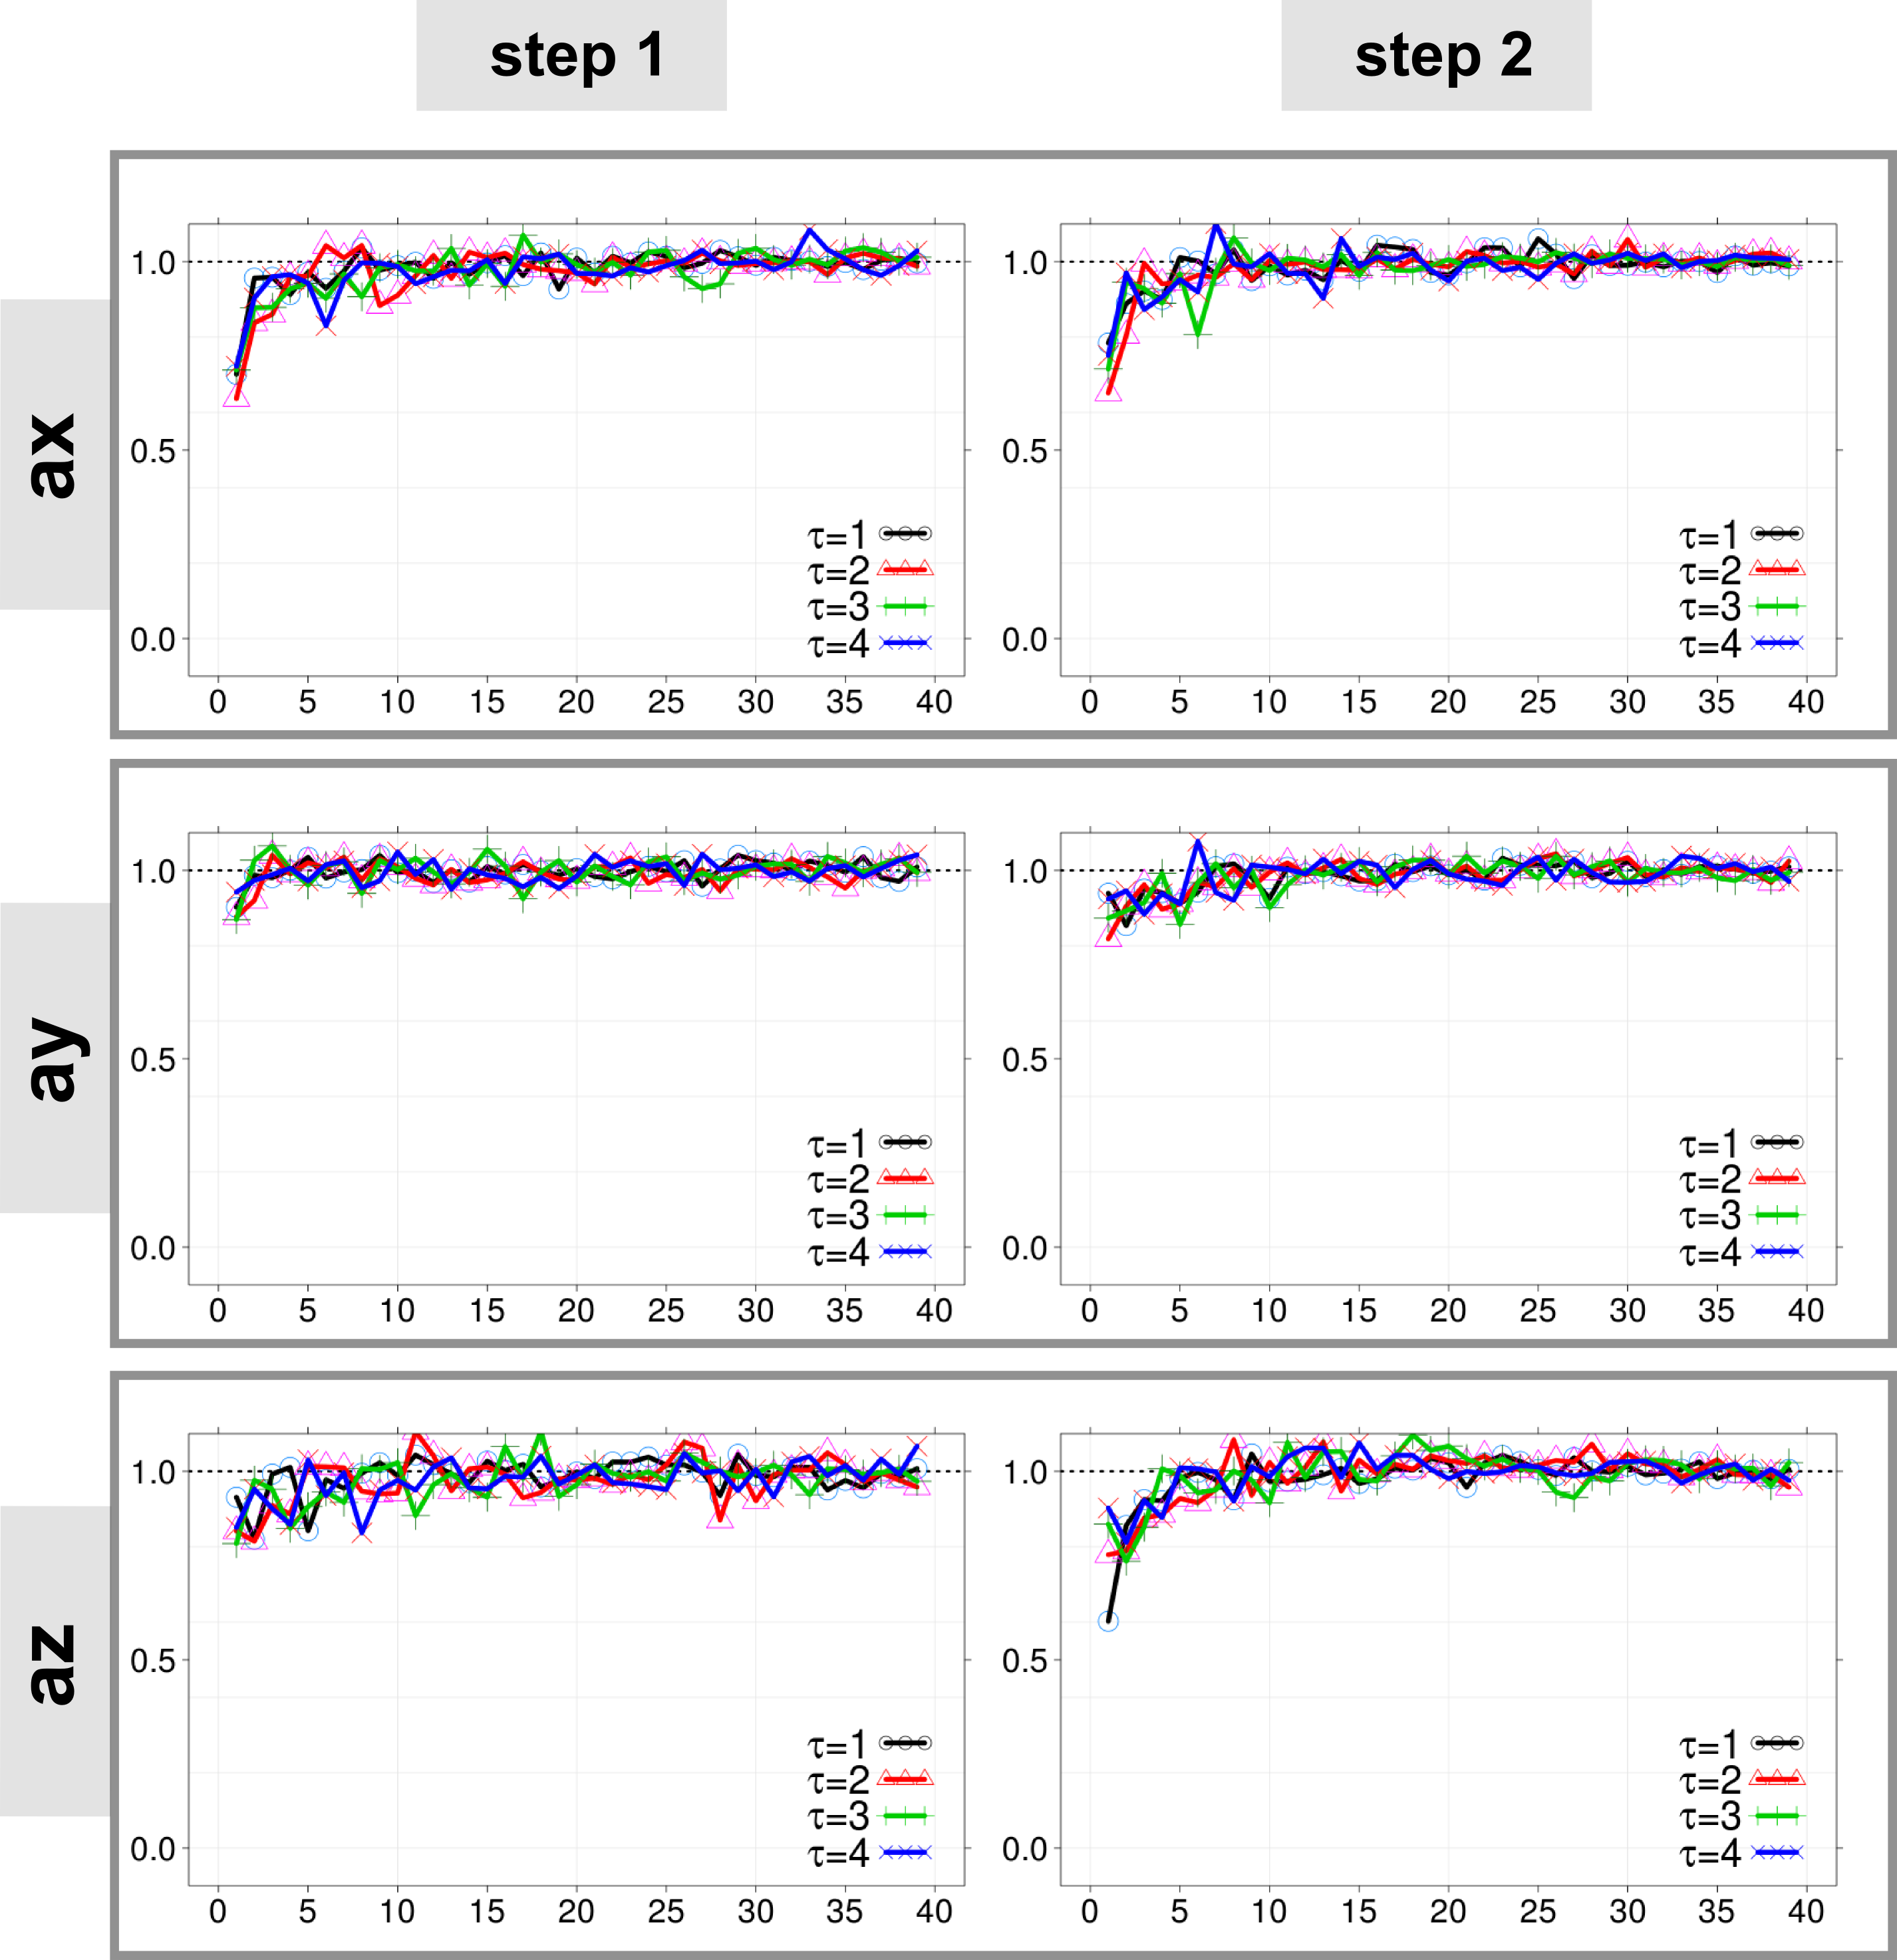
\includegraphics[width=0.45\textwidth]{e2_acc_expert}
  \caption[PA]{$E2(d)$ values for $\tau=1,2,3,4$ with $0 \leq d \leq40 $
  from the triaxial accelerometer of the expert dancer for two steps.
  If $E2(d)$ values are approximately equal to 1 for any $d$ the time serie is random.
  }
  \label{fig:e2acc}
  \end{figure}
  

    \begin{figure}[htbp!] 
  \centering    
  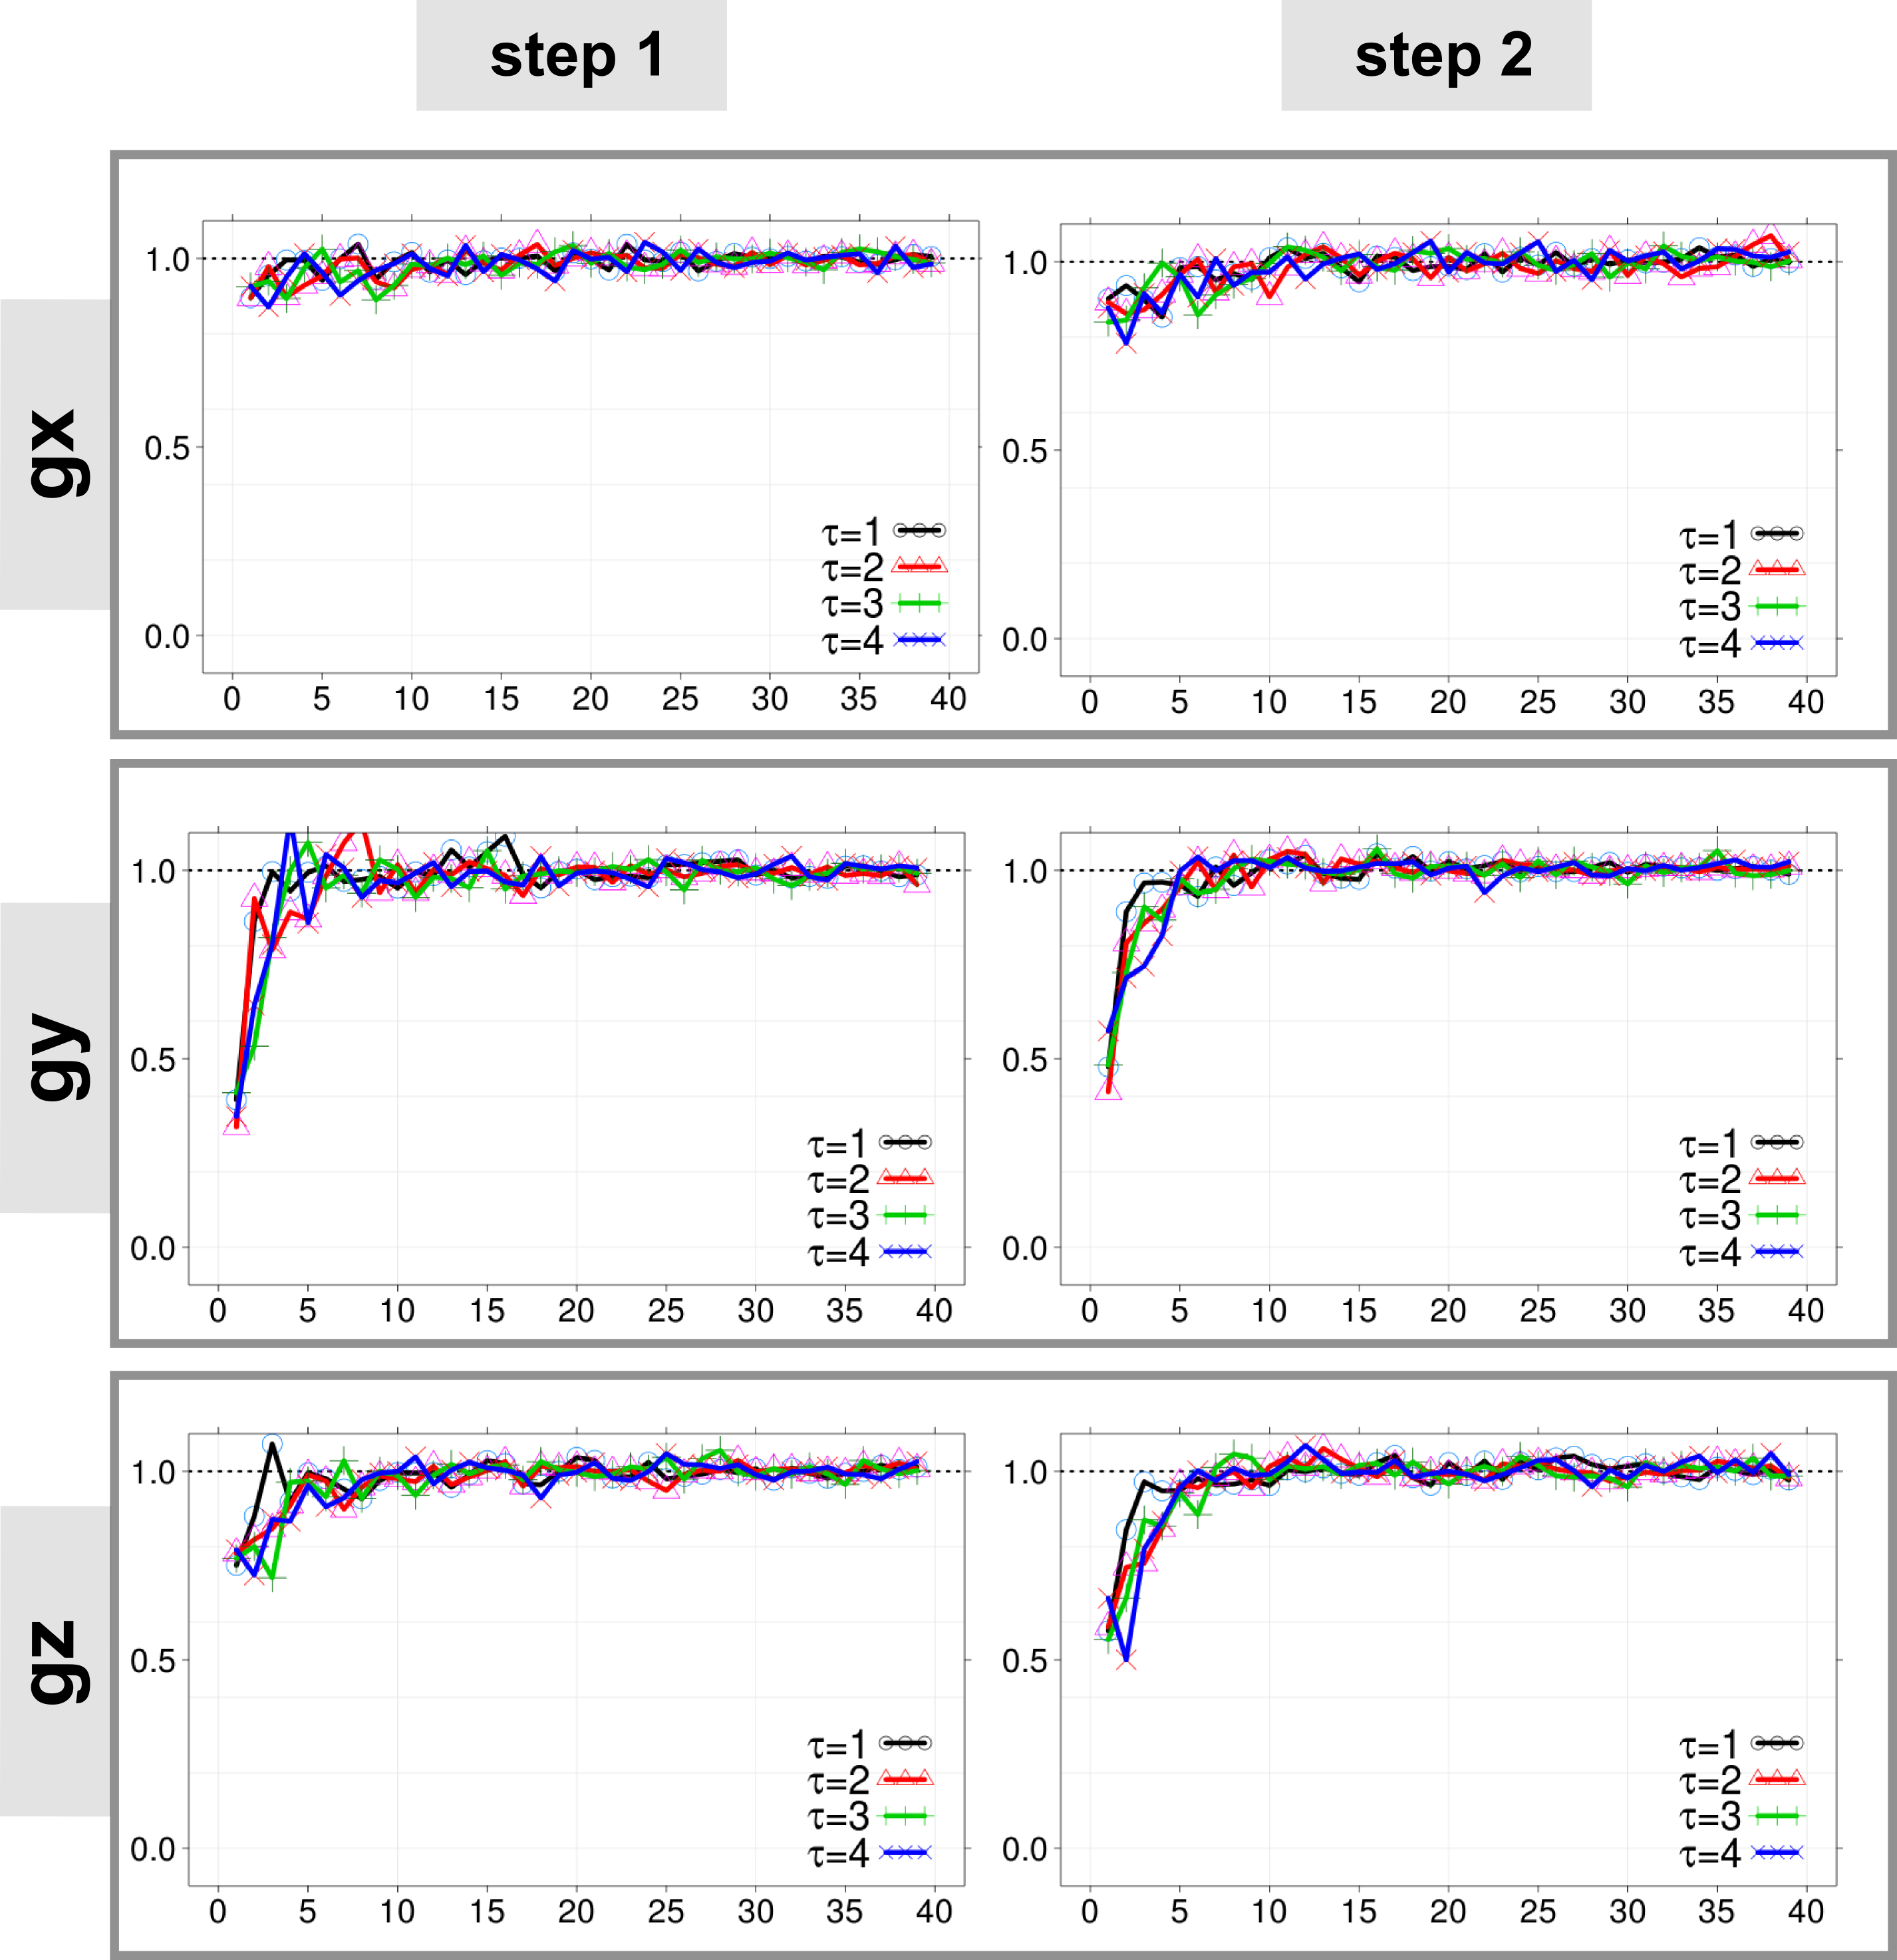
\includegraphics[width=0.45\textwidth]{e2_gyr_expert}
  \caption[PA]{$E2(d)$ values for $\tau=1,2,3,4$ with $0 \leq d \leq40 $
  from the triaxial gyroscope of the expert dancer for two steps.
  If $E2(d)$ values are approximately equal to 1 for any $d$ the time serie is random.
  }
  \label{fig:e2gyr}
  \end{figure}
  
    \begin{figure}[htbp!] 
  \centering    
  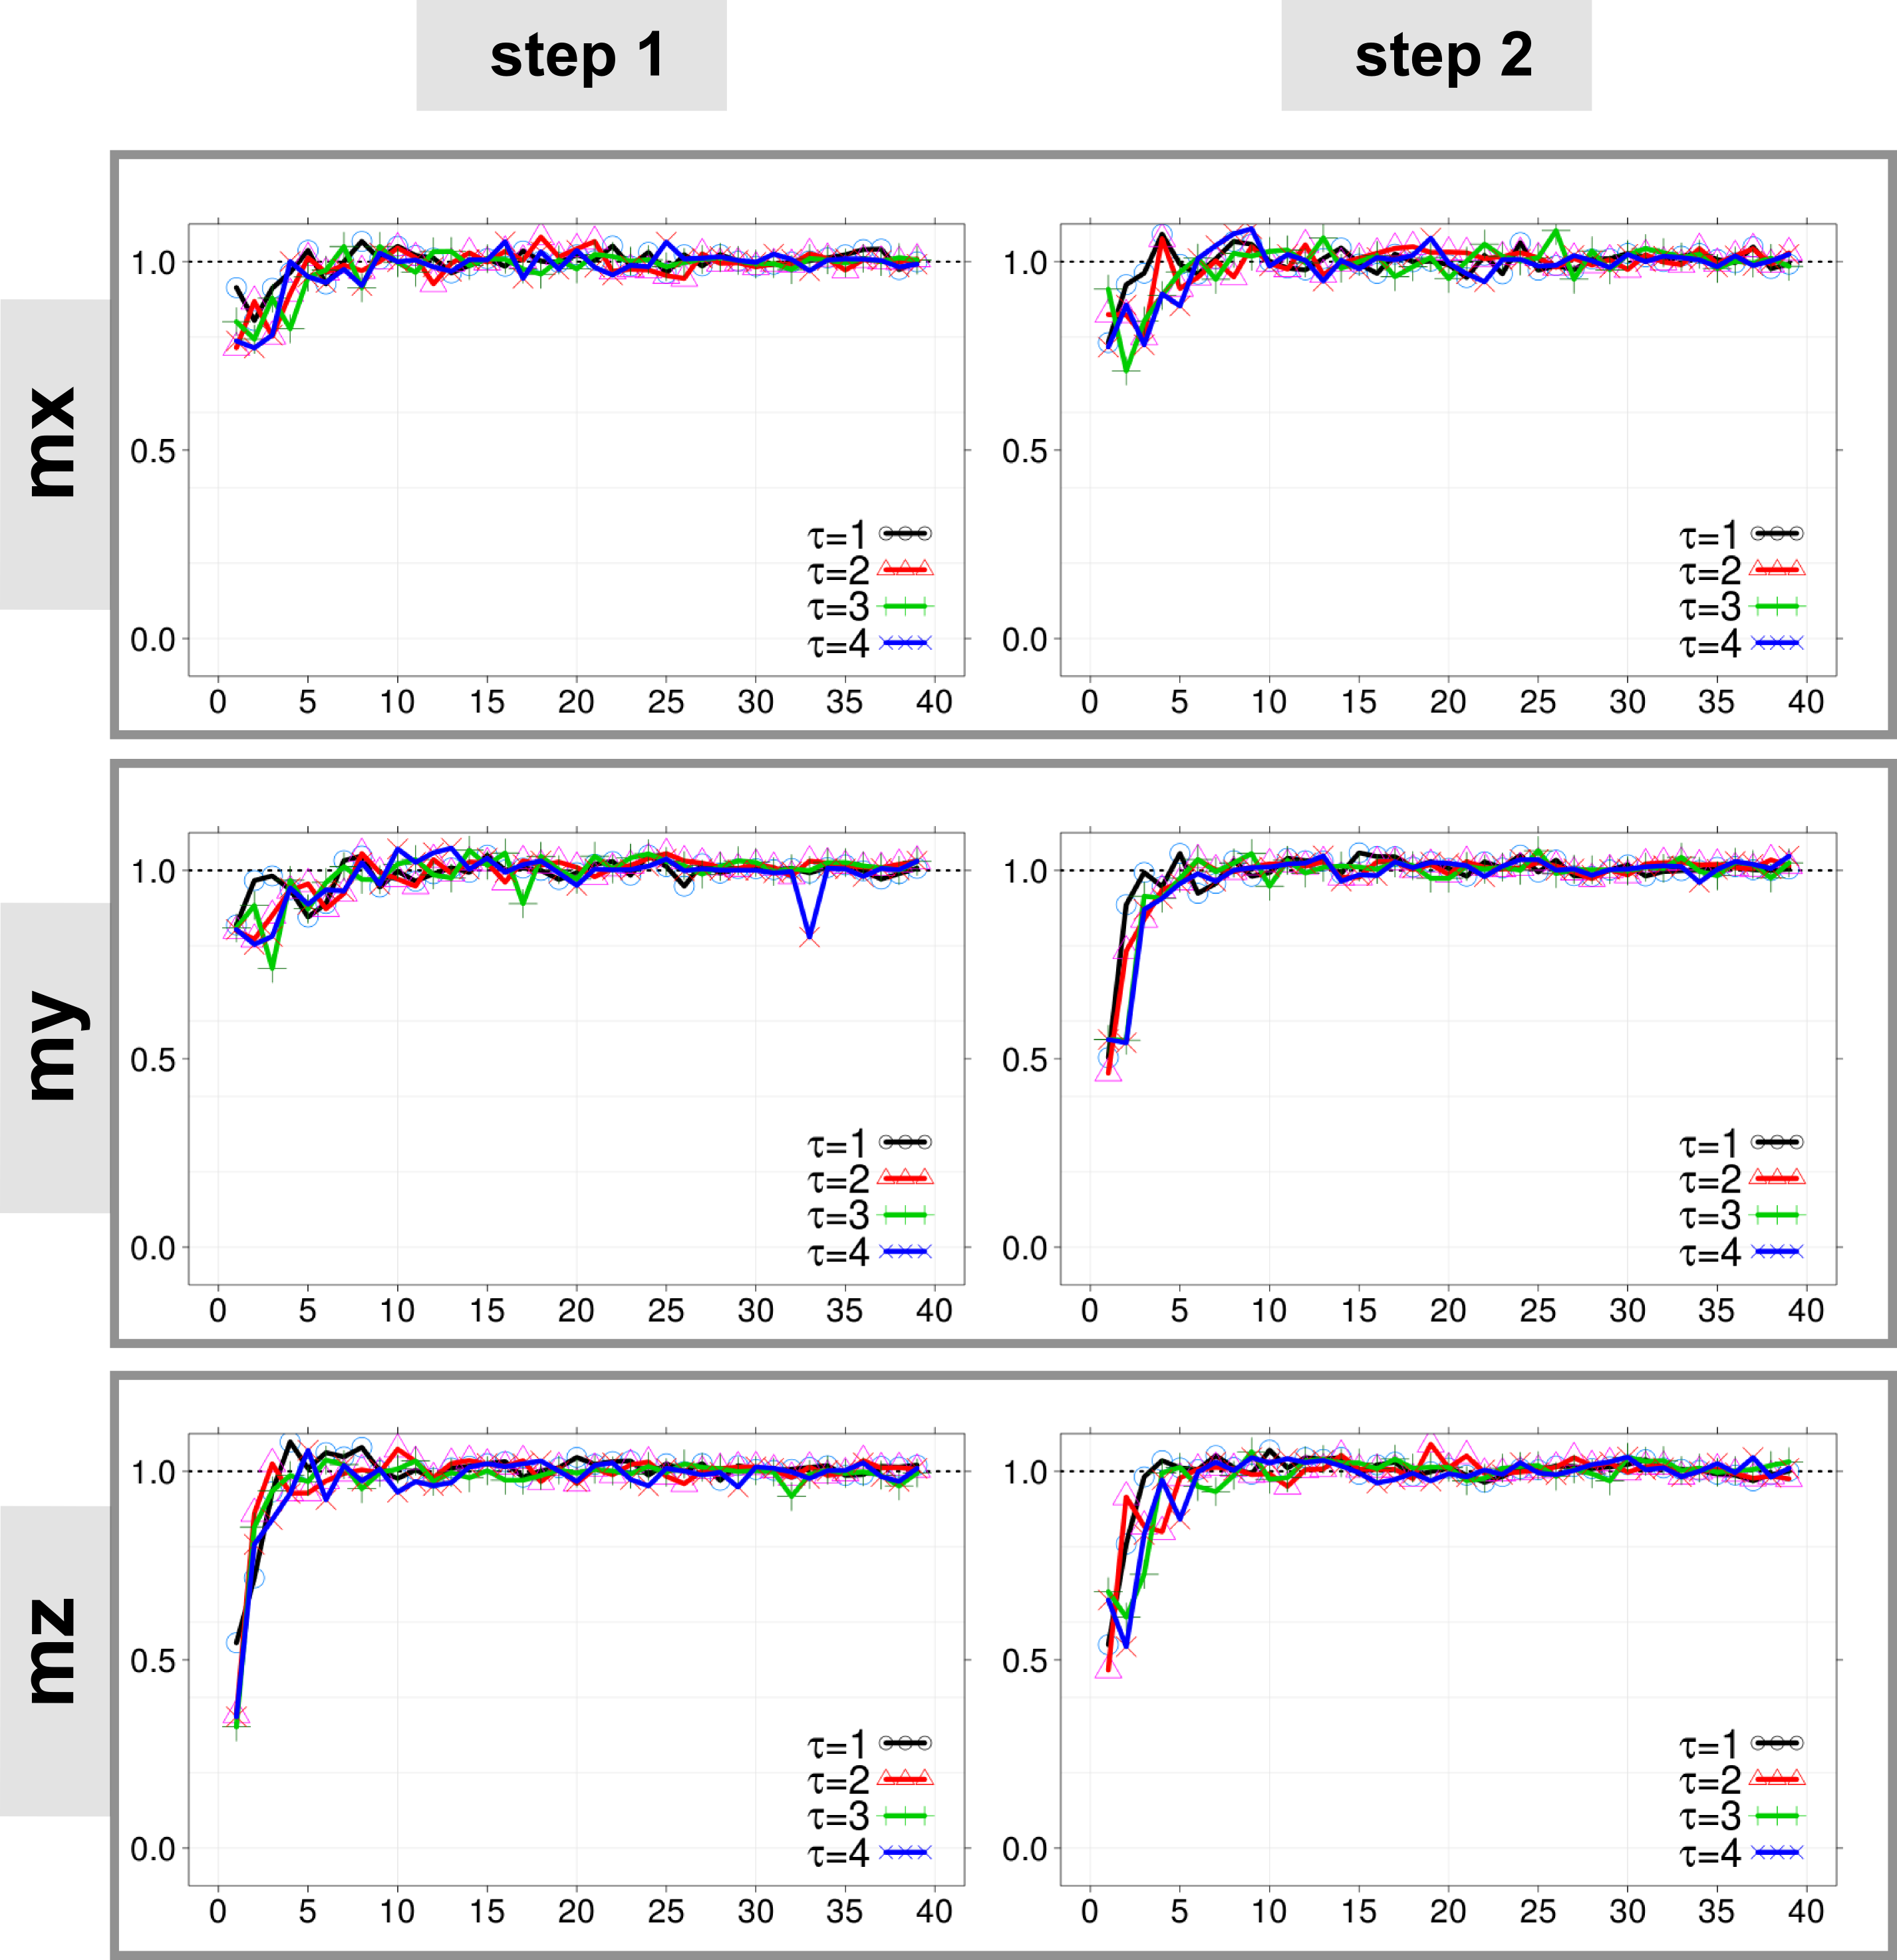
\includegraphics[width=0.45\textwidth]{e2_mag_expert}
  \caption[PA]{$E2(d)$ values for $\tau=1,2,3,4$ with $0 \leq d \leq40 $
  from the triaxial magnetometer of the expert dancer for two steps.
  If $E2(d)$ values are approximately equal to 1 for any $d$ the time serie is random.
  }
  \label{fig:e2mag}
  \end{figure}

  
  \begin{figure}[htbp!] 
  \centering    
  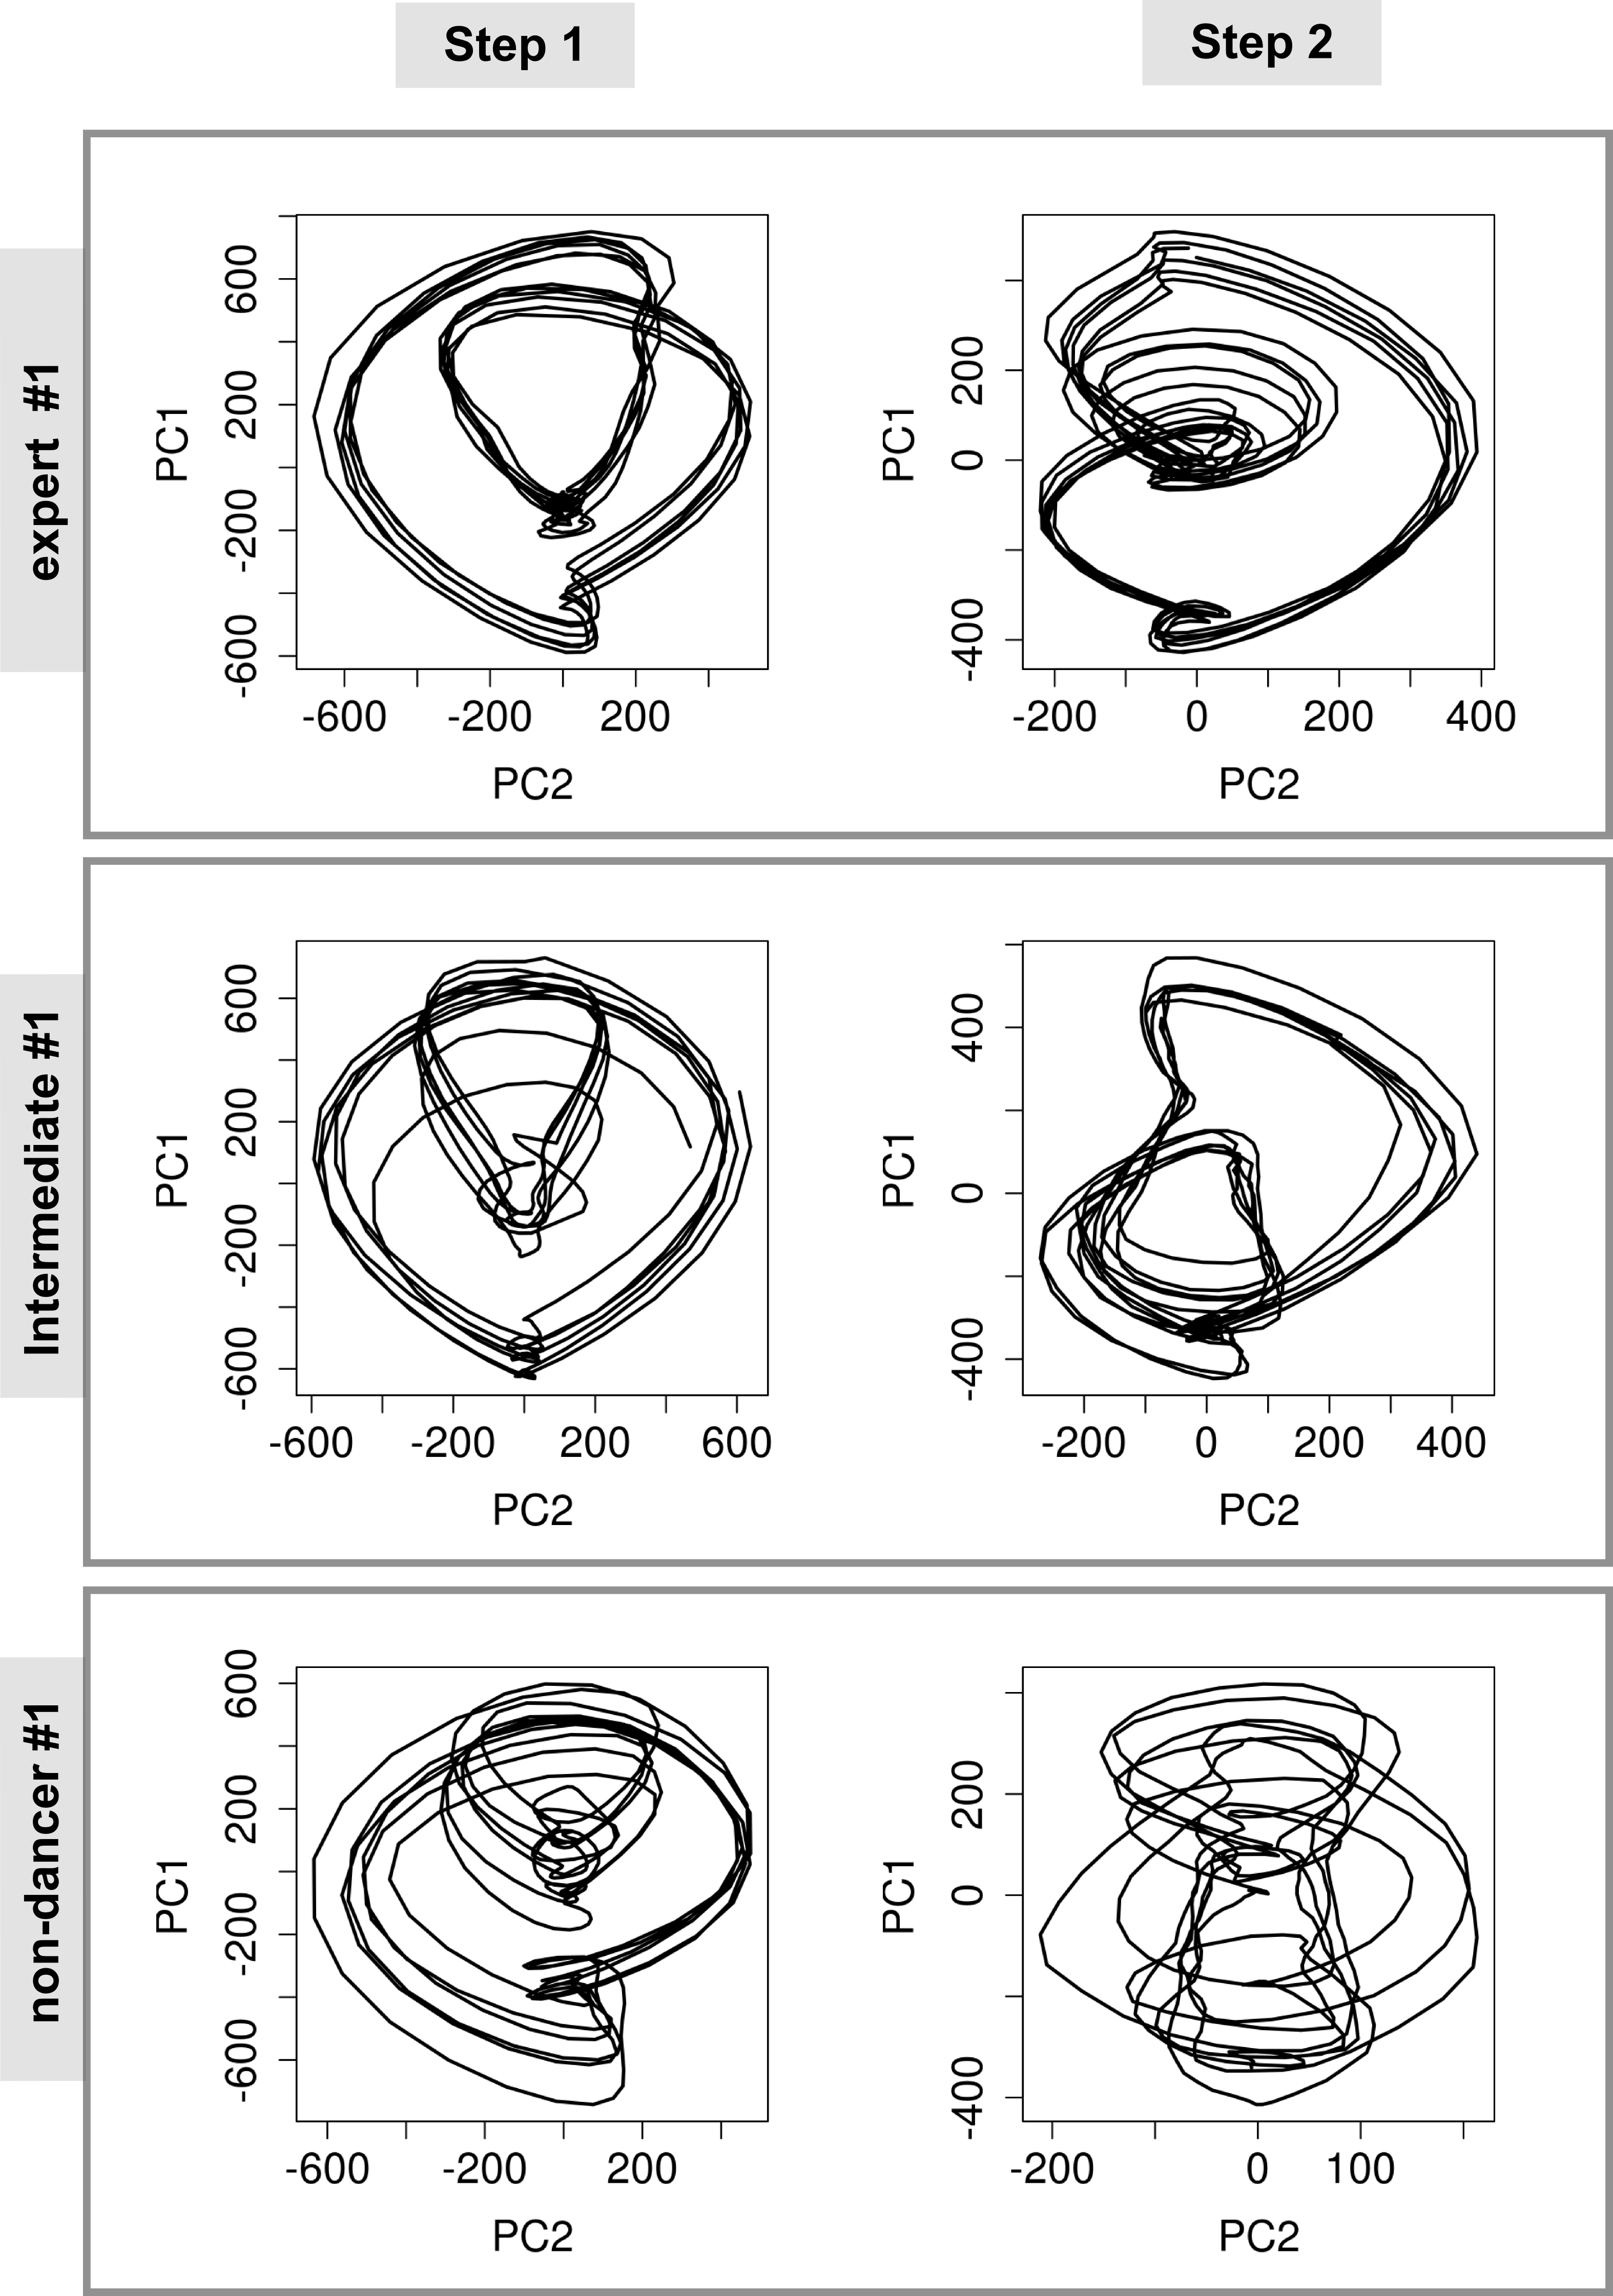
\includegraphics[width=0.45\textwidth]{skills}
  \caption[PA]{2-D reconstructed state spaces for the expert, intermediate and 
  non-dancer participants for two steps. First two component of the PCA
  for with embedding parameters ($m = 10$ and $\tau = 1$).}
  \label{fig:skills}
  \end{figure}


\begin{figure}[htbp!] 
\centering    
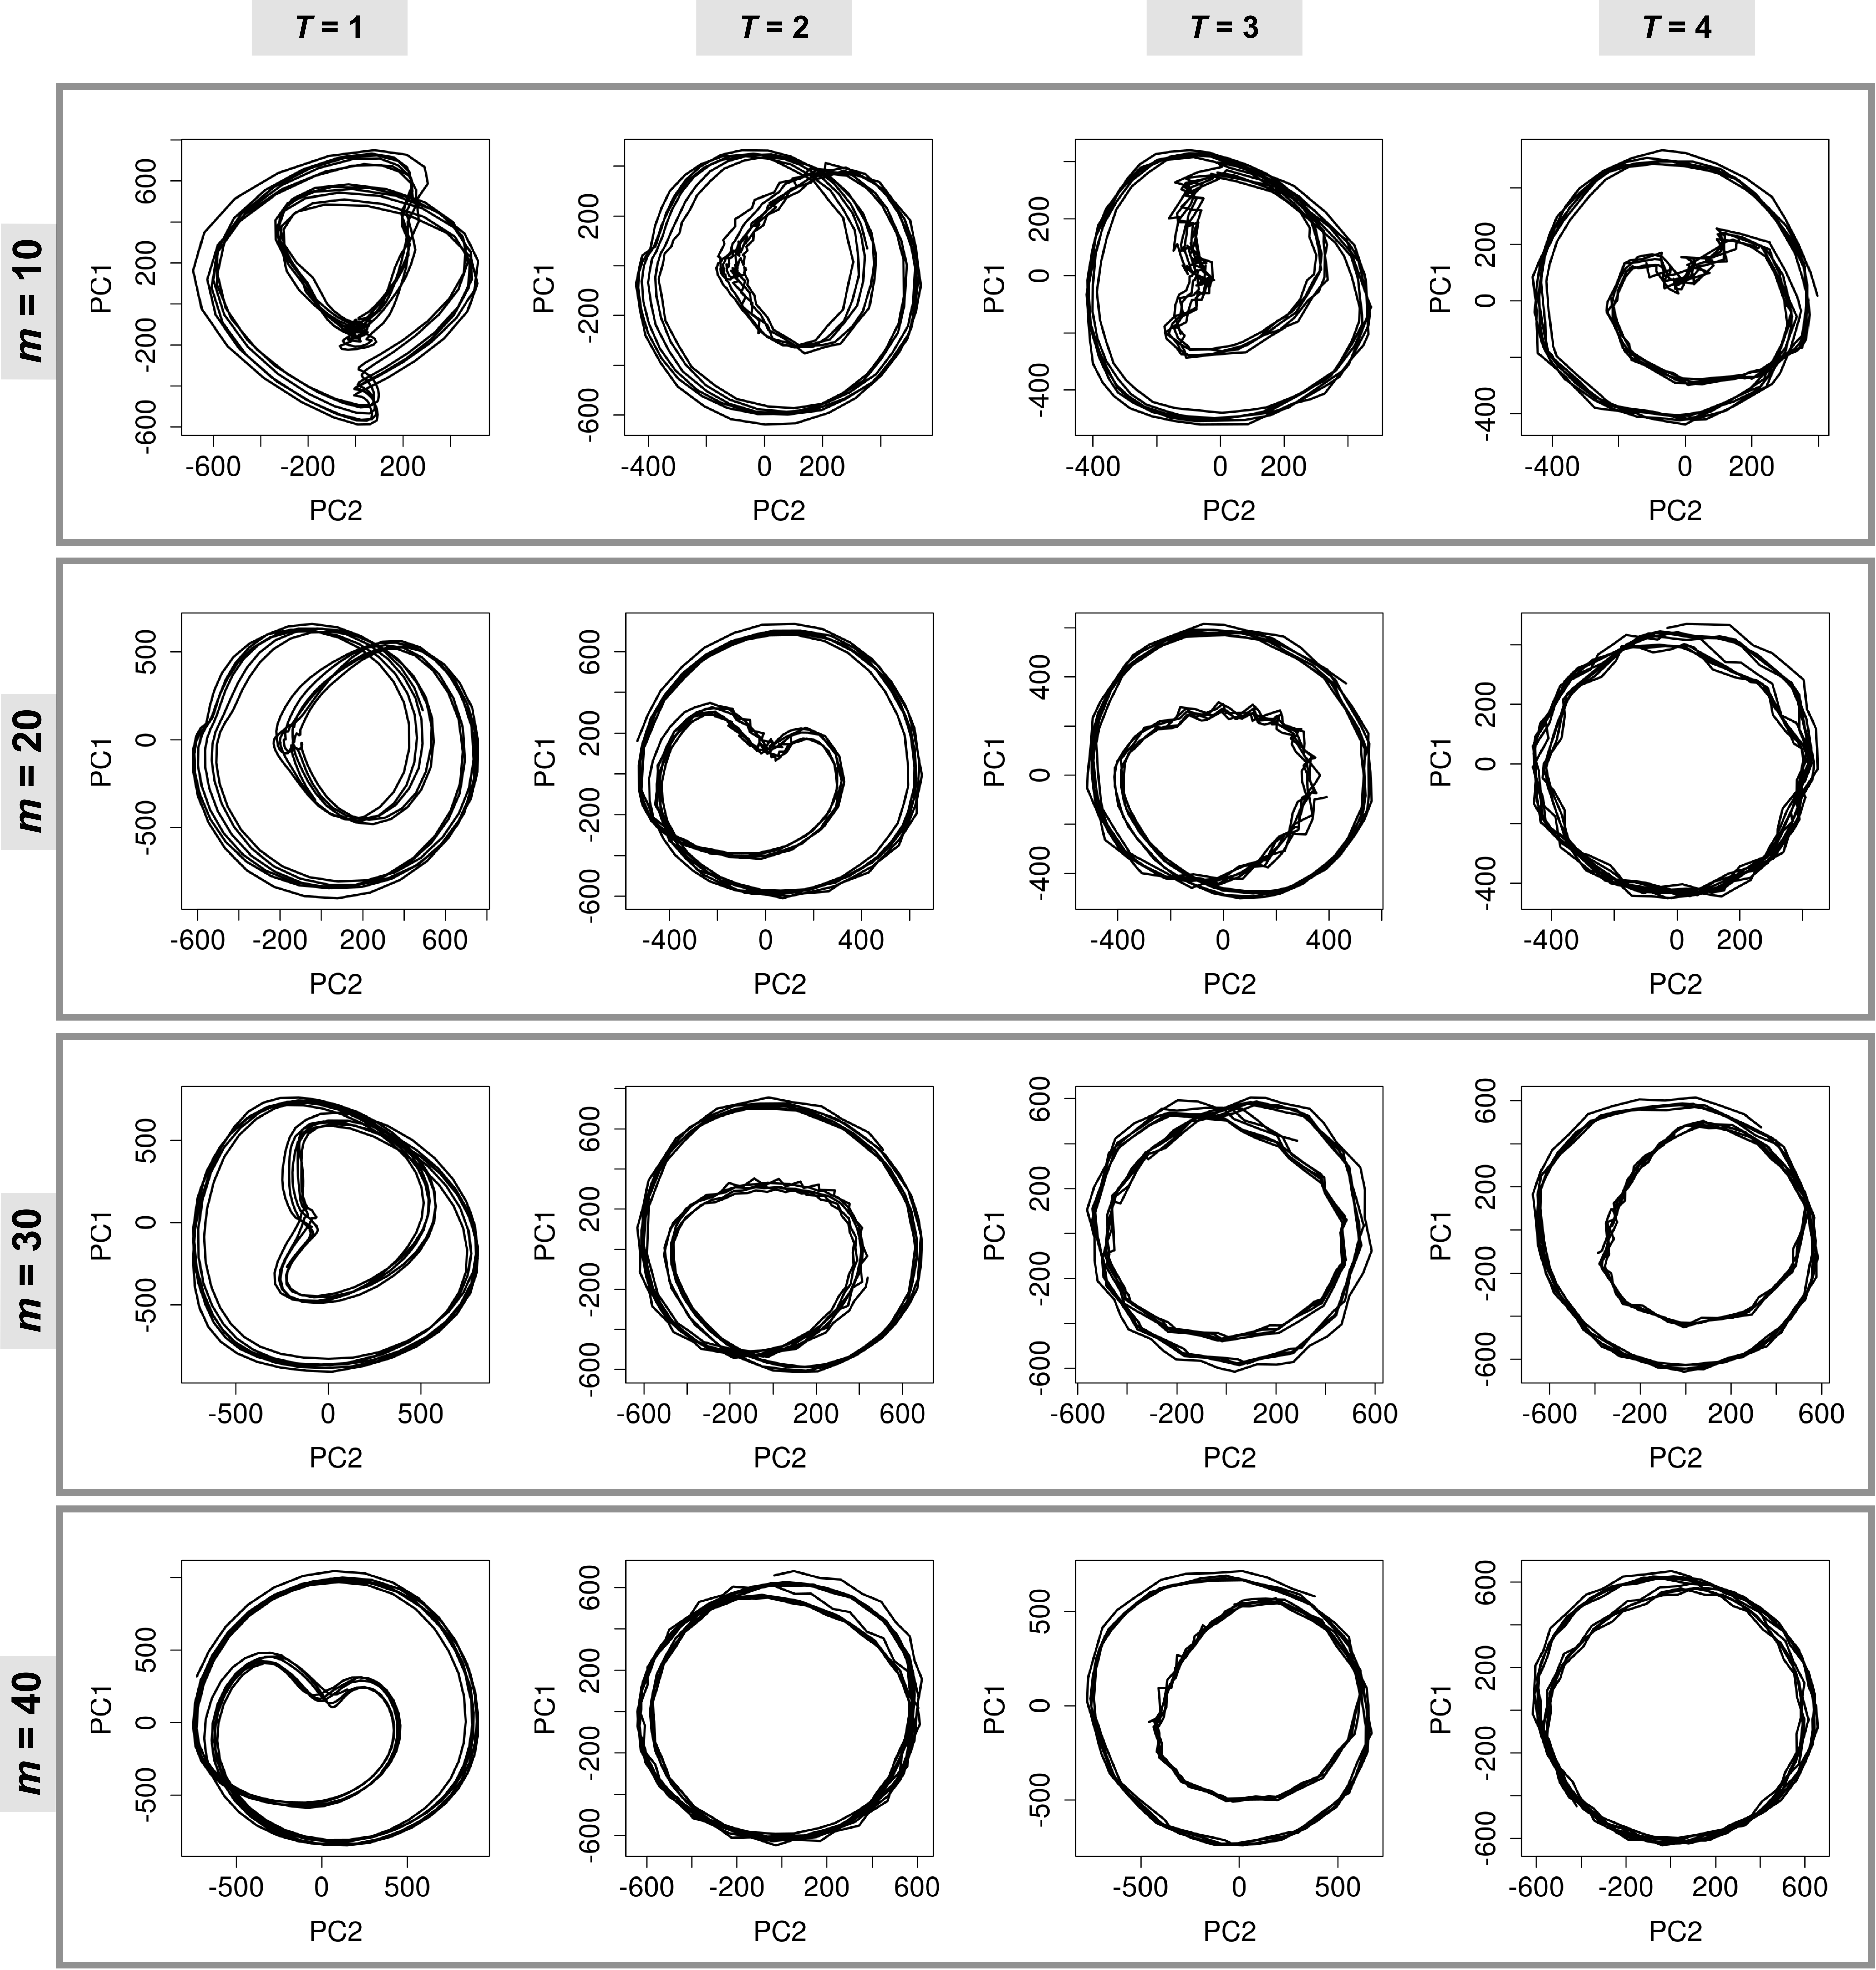
\includegraphics[width=0.45\textwidth]{takens}
\caption[PA]{2-D reconstructed state spaces with different embedded parameters ($m=10,20,30,40$ and $\tau= 1,2,3,4$)
for the same time-serie.}
\label{fig:takens}
\end{figure}



 \section{Conclusion [DRAFT]}
Although the Takens' Theorem is still subjected to the embedded parameters,
the phase space representation applies a model of consistency to the data for skill assessment.
Variability then becomes desiriable because dancers are better able  
to moderate their actions in response to contextual demands.

On the other hand, one can see from the $E2(d)$ values that that accelerometer data 
is more random than the gyroscope and magnetometer data.


 
%  ......................................................................................
% ......................................................................................
% ......................................................................................
% ......................................................................................



Future work, investifate the preservation of geometry \cite{Yap2014} 
for the computation of the minimal embedded parameters.


\section{Acknowledgments}
The authors acknowledge support from 
% Mexico's National Council 
% for Science and Technology, CONACyT, 
% to pursue doctoral research at the 
% University of Birmingham.
% ......................................................................................
% ......................................................................................
% ......................................................................................
% ......................................................................................

% Balancing columns in a ref list is a bit of a pain because you
% either use a hack like flushend or balance, or manually insert
% a column break.  http://www.tex.ac.uk/cgi-bin/texfaq2html?label=balance
% multicols doesn't work because we're already in two-column mode,
% and flushend isn't awesome, so I choose balance.  See this
% for more info: http://cs.brown.edu/system/software/latex/doc/balance.pdf
%
% Note that in a perfect world balance wants to be in the first
% column of the last page.
%
% If balance doesn't work for you, you can remove that and
% hard-code a column break into the bbl file right before you
% submit:
%
% http://stackoverflow.com/questions/2149854/how-to-manually-equalize-columns-
% in-an-ieee-paper-if-using-bibtex
%
% Or, just remove \balance and give up on balancing the last page.
%
\balance



\bibliographystyle{acm-sigchi}
\bibliography{references}
\end{document}
